% Options for packages loaded elsewhere
\PassOptionsToPackage{unicode}{hyperref}
\PassOptionsToPackage{hyphens}{url}
%
\documentclass[
]{book}
\usepackage{amsmath,amssymb}
\usepackage{iftex}
\ifPDFTeX
  \usepackage[T1]{fontenc}
  \usepackage[utf8]{inputenc}
  \usepackage{textcomp} % provide euro and other symbols
\else % if luatex or xetex
  \usepackage{unicode-math} % this also loads fontspec
  \defaultfontfeatures{Scale=MatchLowercase}
  \defaultfontfeatures[\rmfamily]{Ligatures=TeX,Scale=1}
\fi
\usepackage{lmodern}
\ifPDFTeX\else
  % xetex/luatex font selection
\fi
% Use upquote if available, for straight quotes in verbatim environments
\IfFileExists{upquote.sty}{\usepackage{upquote}}{}
\IfFileExists{microtype.sty}{% use microtype if available
  \usepackage[]{microtype}
  \UseMicrotypeSet[protrusion]{basicmath} % disable protrusion for tt fonts
}{}
\makeatletter
\@ifundefined{KOMAClassName}{% if non-KOMA class
  \IfFileExists{parskip.sty}{%
    \usepackage{parskip}
  }{% else
    \setlength{\parindent}{0pt}
    \setlength{\parskip}{6pt plus 2pt minus 1pt}}
}{% if KOMA class
  \KOMAoptions{parskip=half}}
\makeatother
\usepackage{xcolor}
\usepackage{color}
\usepackage{fancyvrb}
\newcommand{\VerbBar}{|}
\newcommand{\VERB}{\Verb[commandchars=\\\{\}]}
\DefineVerbatimEnvironment{Highlighting}{Verbatim}{commandchars=\\\{\}}
% Add ',fontsize=\small' for more characters per line
\usepackage{framed}
\definecolor{shadecolor}{RGB}{248,248,248}
\newenvironment{Shaded}{\begin{snugshade}}{\end{snugshade}}
\newcommand{\AlertTok}[1]{\textcolor[rgb]{0.94,0.16,0.16}{#1}}
\newcommand{\AnnotationTok}[1]{\textcolor[rgb]{0.56,0.35,0.01}{\textbf{\textit{#1}}}}
\newcommand{\AttributeTok}[1]{\textcolor[rgb]{0.13,0.29,0.53}{#1}}
\newcommand{\BaseNTok}[1]{\textcolor[rgb]{0.00,0.00,0.81}{#1}}
\newcommand{\BuiltInTok}[1]{#1}
\newcommand{\CharTok}[1]{\textcolor[rgb]{0.31,0.60,0.02}{#1}}
\newcommand{\CommentTok}[1]{\textcolor[rgb]{0.56,0.35,0.01}{\textit{#1}}}
\newcommand{\CommentVarTok}[1]{\textcolor[rgb]{0.56,0.35,0.01}{\textbf{\textit{#1}}}}
\newcommand{\ConstantTok}[1]{\textcolor[rgb]{0.56,0.35,0.01}{#1}}
\newcommand{\ControlFlowTok}[1]{\textcolor[rgb]{0.13,0.29,0.53}{\textbf{#1}}}
\newcommand{\DataTypeTok}[1]{\textcolor[rgb]{0.13,0.29,0.53}{#1}}
\newcommand{\DecValTok}[1]{\textcolor[rgb]{0.00,0.00,0.81}{#1}}
\newcommand{\DocumentationTok}[1]{\textcolor[rgb]{0.56,0.35,0.01}{\textbf{\textit{#1}}}}
\newcommand{\ErrorTok}[1]{\textcolor[rgb]{0.64,0.00,0.00}{\textbf{#1}}}
\newcommand{\ExtensionTok}[1]{#1}
\newcommand{\FloatTok}[1]{\textcolor[rgb]{0.00,0.00,0.81}{#1}}
\newcommand{\FunctionTok}[1]{\textcolor[rgb]{0.13,0.29,0.53}{\textbf{#1}}}
\newcommand{\ImportTok}[1]{#1}
\newcommand{\InformationTok}[1]{\textcolor[rgb]{0.56,0.35,0.01}{\textbf{\textit{#1}}}}
\newcommand{\KeywordTok}[1]{\textcolor[rgb]{0.13,0.29,0.53}{\textbf{#1}}}
\newcommand{\NormalTok}[1]{#1}
\newcommand{\OperatorTok}[1]{\textcolor[rgb]{0.81,0.36,0.00}{\textbf{#1}}}
\newcommand{\OtherTok}[1]{\textcolor[rgb]{0.56,0.35,0.01}{#1}}
\newcommand{\PreprocessorTok}[1]{\textcolor[rgb]{0.56,0.35,0.01}{\textit{#1}}}
\newcommand{\RegionMarkerTok}[1]{#1}
\newcommand{\SpecialCharTok}[1]{\textcolor[rgb]{0.81,0.36,0.00}{\textbf{#1}}}
\newcommand{\SpecialStringTok}[1]{\textcolor[rgb]{0.31,0.60,0.02}{#1}}
\newcommand{\StringTok}[1]{\textcolor[rgb]{0.31,0.60,0.02}{#1}}
\newcommand{\VariableTok}[1]{\textcolor[rgb]{0.00,0.00,0.00}{#1}}
\newcommand{\VerbatimStringTok}[1]{\textcolor[rgb]{0.31,0.60,0.02}{#1}}
\newcommand{\WarningTok}[1]{\textcolor[rgb]{0.56,0.35,0.01}{\textbf{\textit{#1}}}}
\usepackage{longtable,booktabs,array}
\usepackage{calc} % for calculating minipage widths
% Correct order of tables after \paragraph or \subparagraph
\usepackage{etoolbox}
\makeatletter
\patchcmd\longtable{\par}{\if@noskipsec\mbox{}\fi\par}{}{}
\makeatother
% Allow footnotes in longtable head/foot
\IfFileExists{footnotehyper.sty}{\usepackage{footnotehyper}}{\usepackage{footnote}}
\makesavenoteenv{longtable}
\usepackage{graphicx}
\makeatletter
\def\maxwidth{\ifdim\Gin@nat@width>\linewidth\linewidth\else\Gin@nat@width\fi}
\def\maxheight{\ifdim\Gin@nat@height>\textheight\textheight\else\Gin@nat@height\fi}
\makeatother
% Scale images if necessary, so that they will not overflow the page
% margins by default, and it is still possible to overwrite the defaults
% using explicit options in \includegraphics[width, height, ...]{}
\setkeys{Gin}{width=\maxwidth,height=\maxheight,keepaspectratio}
% Set default figure placement to htbp
\makeatletter
\def\fps@figure{htbp}
\makeatother
\setlength{\emergencystretch}{3em} % prevent overfull lines
\providecommand{\tightlist}{%
  \setlength{\itemsep}{0pt}\setlength{\parskip}{0pt}}
\setcounter{secnumdepth}{5}
\usepackage{booktabs}
\usepackage{amsthm}
\makeatletter
\def\thm@space@setup{%
  \thm@preskip=8pt plus 2pt minus 4pt
  \thm@postskip=\thm@preskip
}
\makeatother
\usepackage{booktabs}
\usepackage{longtable}
\usepackage{array}
\usepackage{multirow}
\usepackage{wrapfig}
\usepackage{float}
\usepackage{colortbl}
\usepackage{pdflscape}
\usepackage{tabu}
\usepackage{threeparttable}
\usepackage{threeparttablex}
\usepackage[normalem]{ulem}
\usepackage{makecell}
\usepackage{xcolor}
\ifLuaTeX
  \usepackage{selnolig}  % disable illegal ligatures
\fi
\usepackage[]{natbib}
\bibliographystyle{apalike}
\usepackage{bookmark}
\IfFileExists{xurl.sty}{\usepackage{xurl}}{} % add URL line breaks if available
\urlstyle{same}
\hypersetup{
  pdftitle={Half-day Workshop on Phylogenetic Comparative Methods},
  pdfauthor={Simon Joly},
  hidelinks,
  pdfcreator={LaTeX via pandoc}}

\title{Half-day Workshop on Phylogenetic Comparative Methods}
\author{Simon Joly}
\date{2024-11-11}

\begin{document}
\maketitle

{
\setcounter{tocdepth}{1}
\tableofcontents
}
\chapter{About}\label{about}

This document consist in an introduction to the comparative methods. It contains theory as well as practical examples in R on Phylogenetic Generalized Least Squares (PGLS). It was developed for a half-day workshop that consists in short presentations followed by R exercises. Note that the present document should pretty much stand by itself because most of the theory given in the presentations are incorporated into the theory sections. Therefore, this document should contain all the necessary information to understand the examples.

I assume that the readers are ``reasonably'' familiar with R as well as with linear regression and its assumptions. There are a lot of good R introductory tutorials on the web and for linear models. Zuur et al. \citep{zuur2007analysing} provide a good introduction to linear models, mixed-effects models and model comparison. Good introductions to model fitting in R can also be found on Dolph Schluter's \href{https://www.zoology.ubc.ca/~schluter/R/fit-model/}{webpage} and among the \href{http://qcbs.ca/wiki/r_workshop4}{QCBS workshops}.

\section{Useful resources}\label{useful-resources}

The links below might provide additional information of interest.

Luke Harmon's book - \href{https://lukejharmon.github.io/pcm/}{Phylogenetic Comparative Methods}

Liam Revell's \href{http://blog.phytools.org/}{blog on phylogenetic tools in R}

Liam Revell and Luke Harmon \href{https://press.princeton.edu/books/ebook/9780691219042/phylogenetic-comparative-methods-in-r}{book on Phylogenetic comparative methods in R}

The list of \href{https://cran.r-project.org/web/views/Phylogenetics.html}{R packages for phylogenies}

\href{http://github.com/simjoly/CourseComparativeMethods/}{My tutorials on Phylogenetic Comparative Methods}

R package \href{https://doi.org/10.1016/j.pld.2022.05.005}{V.PhyloMaker2} that can generate very large phylogenies for vascular plants and R package \href{https://doi.org/10.1016/j.pld.2022.12.007}{U.PhyloMaker} that can generate large phylogenetic trees for plants and animals

\section{Source}\label{source}

This tutorial is publicly available and is hosted on github in the repository \href{https://github.com/simjoly/ComparativeMethods-HalfDayWorkshop}{github.com/simjoly/ComparativeMethods-HalfDayWorkshop}

\section{Disclaimer}\label{disclaimer}

This tutorial is provided as is, without any guaranty that it will work or that the analyses will be up to date.

\chapter{Ahead of the workshop}\label{before}

Here are a few things you should know and you should do ahead of the workshop.

\section{Install R and the required packages}\label{install-r-and-the-required-packages}

To perform the examples of this document, you will need to have the \href{https://www.r-project.org/}{R software} installed on your computer. I strongly recommend that you install \href{https://rstudio.com/}{RStudio}. Although R Studio is not required, it facilitates interactions between scripts and the R console and provides many great tools.

After installing R, you will have to install some packages. For this specific tutorial, we will need to load the following R packages.

\begin{Shaded}
\begin{Highlighting}[]
\FunctionTok{library}\NormalTok{(nlme)}
\FunctionTok{library}\NormalTok{(ape)}
\FunctionTok{library}\NormalTok{(RColorBrewer)}
\FunctionTok{library}\NormalTok{(ggplot2)}
\end{Highlighting}
\end{Shaded}

To execute the code of this tutorial in R, I suggest that you create a new script (File\textgreater New File\textgreater R Script) where you paste the code copied from the boxes. In R Studio, you can then run this code by selecting the lines you want to execute and then press run (or associated shortcut). This will replicate the analyses presented in the tutorial. You should save the script file in a directory dedicated for the workshop where you will also place the data files required (see section \ref{download}). Then, you should make sure that you script (and data) are in the R working directory. In R Studio, this can be set form the menu: `Session \textgreater{} Set Working Directory'.

If some of the packages above are not yet installed on your computer, you get error messages when trying to load them. If this is the case, you will have to install them using the function \texttt{install.packages()}. You only have to install them only once.

\begin{Shaded}
\begin{Highlighting}[]
\FunctionTok{install.packages}\NormalTok{(}\StringTok{\textquotesingle{}nlme\textquotesingle{}}\NormalTok{)}
\FunctionTok{install.packages}\NormalTok{(}\StringTok{\textquotesingle{}ape\textquotesingle{}}\NormalTok{)}
\FunctionTok{install.packages}\NormalTok{(}\StringTok{\textquotesingle{}RColorBrewer\textquotesingle{}}\NormalTok{)}
\FunctionTok{install.packages}\NormalTok{(}\StringTok{\textquotesingle{}ggplot2\textquotesingle{}}\NormalTok{)}
\end{Highlighting}
\end{Shaded}

Once the packages are installed, you can load the packages using the \texttt{library()} function. Also note that if you are using both the packages \texttt{nlme} and \texttt{ape}, \texttt{nlme} should be loaded first. If you don't do this, you might get errors; you could then restart R and start over.

\section{Downloading the data}\label{download}

The data you will need for this tutorial can be downloaded from this repository: \href{https://simjoly.github.io/ComparativeMethods-HalfDayWorkshop/data.zip}{data.zip}.

I suggest that you download the folder, uncompress it, and place is in a dedicated folder where you will also save the script with all the commands you will use.

\section{Get acquainted with phylogenetic trees in R}\label{get-acquainted-with-phylogenetic-trees-in-r}

I you never used phylogenetic trees in R, you can learn some basic techniques on how to handle them and simulate trees and characters by reading chapter \ref{trees}.

\chapter{An introduction to Phylogenetic Comparative Methods}\label{intro}

Phylogenetic comparative methods were introduced by Joseph Felsenstein in 1985. The idea of phylogenetic comparative methods was to correct for the non-independence of species in statistical tests because of their shared evolutionary histories. Indeed, two species may look similar not because they live in the same environment but because they are closely related. Consider the following angiosperm phylogeny.

\begin{figure}

{\centering 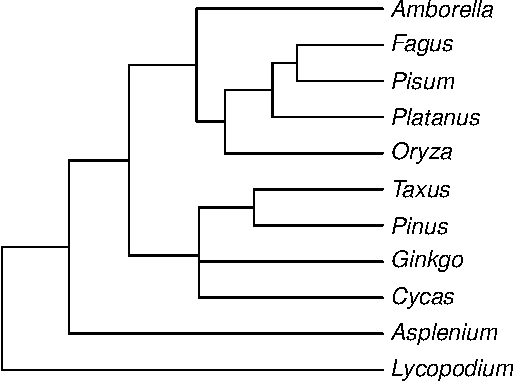
\includegraphics{pcm-workshop_files/figure-latex/AngiospermTree-1} 

}

\caption{land plant phylogeny}\label{fig:AngiospermTree}
\end{figure}

It is clear that \emph{Fagus} (beech) and \emph{Pisum} (pea) are more likely to share similar characteristics compared to \emph{Asplenium} (a fern), because they share a more recent common ancestor. In other words, their evolutionary histories are shared over a longer period than with \emph{Asplenium}. As such, they have more chance to have more similar traits (and in fact they do). For instance, take two characters, ovule and fertilization type, within this group.

\begin{center}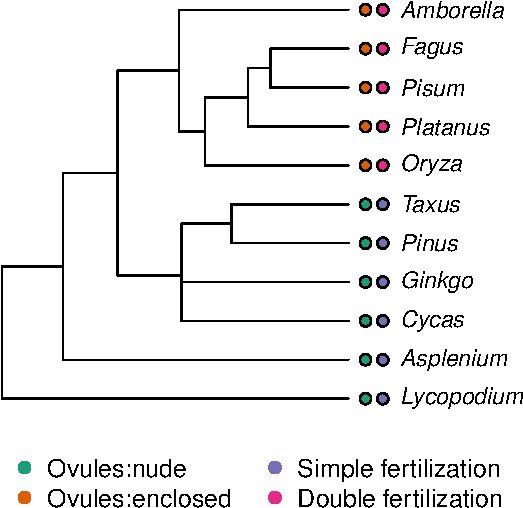
\includegraphics{pcm-workshop_files/figure-latex/AngiospermsWithCharacters-1} \end{center}

Ignoring the phylogeny, we might be tempted to see a strong correlation between these two characters. Indeed, the states between the two characters show a perfect correspondence. Using standard contingency table statistics, we could do a Fisher exact test:

\begin{Shaded}
\begin{Highlighting}[]
\FunctionTok{fisher.test}\NormalTok{(}\FunctionTok{matrix}\NormalTok{(}\FunctionTok{c}\NormalTok{(}\DecValTok{5}\NormalTok{,}\DecValTok{0}\NormalTok{,}\DecValTok{0}\NormalTok{,}\DecValTok{6}\NormalTok{),}\AttributeTok{ncol=}\DecValTok{2}\NormalTok{))}
\end{Highlighting}
\end{Shaded}

\begin{verbatim}
## 
##  Fisher's Exact Test for Count Data
## 
## data:  matrix(c(5, 0, 0, 6), ncol = 2)
## p-value = 0.002165
## alternative hypothesis: true odds ratio is not equal to 1
## 95 percent confidence interval:
##  2.842809      Inf
## sample estimates:
## odds ratio 
##        Inf
\end{verbatim}

The test suggests that the assotiation is highly significant. However, we know that the comparisons made are not completely independent. Actually, both characters evolved only once, and this along the same branch.

A more appropriate way to frame the question would be ``what is the probability that two characters evolved along the same branch?''. This can also be calculated using a contingency table, but this time taking the branches of the phylogeny as the units of observation.

In the example, there are 18 branches and the two characters evolved only once and on the same branch. The contingency table when considering the changes along the branches looks like this:

\begin{tabular}{>{}l|r|r}
\hline
  & Change in trait 2 & No change in trait 2\\
\hline
\textbf{Change in trait 1} & 1 & 0\\
\hline
\textbf{No change in trait 1} & 0 & 17\\
\hline
\end{tabular}

With this table, Fisher's exact test will give the following result:

\begin{Shaded}
\begin{Highlighting}[]
\FunctionTok{fisher.test}\NormalTok{(}\FunctionTok{matrix}\NormalTok{(}\FunctionTok{c}\NormalTok{(}\DecValTok{1}\NormalTok{,}\DecValTok{0}\NormalTok{,}\DecValTok{0}\NormalTok{,}\DecValTok{17}\NormalTok{),}\AttributeTok{ncol=}\DecValTok{2}\NormalTok{))}
\end{Highlighting}
\end{Shaded}

\begin{verbatim}
## 
##  Fisher's Exact Test for Count Data
## 
## data:  matrix(c(1, 0, 0, 17), ncol = 2)
## p-value = 0.05556
## alternative hypothesis: true odds ratio is not equal to 1
## 95 percent confidence interval:
##  0.4358974       Inf
## sample estimates:
## odds ratio 
##        Inf
\end{verbatim}

You can see that the result is no longer significant.

While this approach for taking into account the phylogenetic relationships is correct, more powerful comparative methods have been developed. One useful and powerful approach is the Phylogenetic Generalized Least Squares (PGLS). But before we introduce PGLS, we do some revision and look briefly at the standard regression.

\chapter{The linear regression model}\label{linear-regression}

\section{Theory}\label{theory}

The linear model has the following form:

\[\textbf{y} = \alpha + \beta \textbf{x} + \textbf{e}\]

\(\textbf{y}\) is the response (or dependent) variable, \(\textbf{x}\) is the explanatory (or independent) variable, and \(\textbf{e}\) represent the residuals or in other words the variation not explained by the model. For a simple linear regression model, this represents the distance between the observations (i.e., the real data) and the regression line (i.e., the prediction of the model) along the \(y\) axis. The parameters \(\alpha\) represents the intercept, which is the \(y\) value where the regression line crosses the \(y\) axis, whereas the parameter \(\beta\) represent the slope of the line. In practice, you take a sample of size \(N\) and you get estimates \(\hat{\alpha}\) and \(\hat{\beta}\) for the intercept and the slope, respectively. When the linear regression is fitted using ordinary least squares (OLS), the residuals \(\textbf{e}\) are assumed to be normally distributed with an expectation \(0\) and variance \(\sigma^2\). In mathematical terms, \(\textbf{e} \sim N(0,\sigma^2)\).

Obtaining reliable estimates with a linear regression implies that the data meets several assumptions, amongst which are normality, homogeneity, fixed \(X\), independence, and correct model specification. We won't review all these here, but we will focus on one that is often violated when the data are phylogenetically structured, which is \textbf{independence}. This assumption is important as a lack of independence invalidates important tests such as the F-test and the t-test.

You get a violation of independence when the \(\textbf{y}_i\) value at \(\textbf{x}_i\) is influenced by other \(\textbf{x}_i\). Obviously, this can happen with phylogenetically structured data as a response variable is be more likely to react similarly in closely related species because they share many characters by decent. In other words, the \(y\) value for a species in not completely independent from the \(y\) value of a closely related species: their \(y\) are correlated. We'll illustrate this in an example below.

\section{Practice}\label{practice}

To provide pratical examples in this workshop, we will use a dataset of tree functional traits from the province of Quebec \citep{paquette2015explaining}. The dataset consists in a number of plant functional traits and in a molecular phylogeny built using the plant barcode markers \emph{rbc}L and \emph{mat}K. The dataset you need to run the examples are already in the /data/ folder of the github repository. However, you can also download them by clicking on the links below.

\href{https://simjoly.github.io/ComparativeMethods-HalfDayWorkshop/data/seedplants.tre}{seedplants.tre}

\href{https://simjoly.github.io/ComparativeMethods-HalfDayWorkshop/data/seedplants.csv}{seedplants.csv}

Before analysing the data, we will start by opening the data and the phylogenetic tree and clean them to keep only the species present in both the tree and the trait table. This is necessary because some additional species were included in the phylogenetic tree analysis.

\begin{Shaded}
\begin{Highlighting}[]
\FunctionTok{require}\NormalTok{(ape)}
\CommentTok{\# Open the documents; it assumes that you are in the main directory of the workshop folder}
\NormalTok{seedplantstree }\OtherTok{\textless{}{-}} \FunctionTok{read.nexus}\NormalTok{(}\StringTok{"./data/seedplants.tre"}\NormalTok{)}
\NormalTok{seedplantsdata }\OtherTok{\textless{}{-}} \FunctionTok{read.csv2}\NormalTok{(}\StringTok{"./data/seedplants.csv"}\NormalTok{)}
\CommentTok{\# Remove species for which we don\textquotesingle{}t have complete data}
\NormalTok{seedplantsdata }\OtherTok{\textless{}{-}} \FunctionTok{na.omit}\NormalTok{(seedplantsdata)}
\CommentTok{\# Remove species in the tree that are not in the data matrix}
\NormalTok{species.to.exclude }\OtherTok{\textless{}{-}}\NormalTok{ seedplantstree}\SpecialCharTok{$}\NormalTok{tip.label[}\SpecialCharTok{!}\NormalTok{(seedplantstree}\SpecialCharTok{$}\NormalTok{tip.label }\SpecialCharTok{\%in\%}\NormalTok{ seedplantsdata}\SpecialCharTok{$}\NormalTok{Code)]}
\NormalTok{seedplantstree }\OtherTok{\textless{}{-}} \FunctionTok{drop.tip}\NormalTok{(seedplantstree,species.to.exclude)}
\CommentTok{\# Remove unnecessary object}
\FunctionTok{rm}\NormalTok{(species.to.exclude)}
\CommentTok{\# Order the tree to make it nicer when plotting}
\NormalTok{seedplantstree }\OtherTok{\textless{}{-}} \FunctionTok{ladderize}\NormalTok{(seedplantstree, }\AttributeTok{right =} \ConstantTok{FALSE}\NormalTok{)}
\CommentTok{\# Now let\textquotesingle{}s look at the tree}
\FunctionTok{plot}\NormalTok{(seedplantstree,}\AttributeTok{cex=}\FloatTok{0.4}\NormalTok{)}
\end{Highlighting}
\end{Shaded}

\begin{center}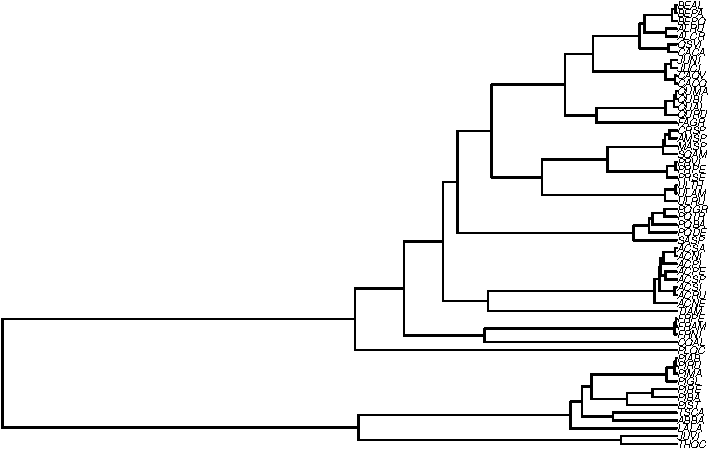
\includegraphics{pcm-workshop_files/figure-latex/Open_seed_plant_data-1} \end{center}

Now, we can have a look at the data, and then order the plant trait to be in the same order as the species in the tree.

\begin{Shaded}
\begin{Highlighting}[]
\CommentTok{\# Here is what the loaded data looks like}
\FunctionTok{head}\NormalTok{(seedplantsdata)}
\end{Highlighting}
\end{Shaded}

\begin{verbatim}
##   Code       Species.name Occurrence maxH   Wd    Sm Shade    N
## 1 ABBA     Abies balsamea       7759   25 0.34   7.6   5.0 1.66
## 2 ACNE       Acer negundo          0   20 0.44  34.0   3.5 2.50
## 3 ACNI        Acer nigrum          1   30 0.52  65.0   3.0 1.83
## 4 ACPE Acer pensylvanicum        665   10 0.44  41.0   3.5 2.22
## 5 ACPL   Acer platanoides          0   15 0.51 172.0   4.2 1.99
## 6 ACRU        Acer rubrum       3669   25 0.49  20.0   3.4 1.91
\end{verbatim}

\begin{Shaded}
\begin{Highlighting}[]
\CommentTok{\# Name the rows of the data.frame with the species codes used as tree labels }
\FunctionTok{rownames}\NormalTok{(seedplantsdata) }\OtherTok{\textless{}{-}}\NormalTok{ seedplantsdata}\SpecialCharTok{$}\NormalTok{Code}
\CommentTok{\# Order the data in the same order as the tip.label of the tree. In the present }
\CommentTok{\#  example, this was already the case, but it is an important step for }
\CommentTok{\#  any analysis.}
\NormalTok{seedplantsdata }\OtherTok{\textless{}{-}}\NormalTok{ seedplantsdata[seedplantstree}\SpecialCharTok{$}\NormalTok{tip.label,]}
\end{Highlighting}
\end{Shaded}

Now that the data is ready, let's fit a linear model and try to explain shade tolerance (Shade) of trees using wood density (Wd). In R, a very simple way to do a regression is to use the function `lm', which stands for linear model. To fit a linear model, you need to tell the \texttt{lm} function which variable is the response variable and which one is the explanatory variable. This is done using formulas in the form \texttt{Shade\ \textasciitilde{}\ Wd}. The variable at the left of the tilde (`\textasciitilde{}') is the response variable (\texttt{Shade}) whereas the explanatory variale (1 or more) are at the right of the tilde.

\begin{Shaded}
\begin{Highlighting}[]
\CommentTok{\# Fit a linear model using Ordinary Least Squares (OLS)}
\NormalTok{shade.lm }\OtherTok{\textless{}{-}} \FunctionTok{lm}\NormalTok{(Shade }\SpecialCharTok{\textasciitilde{}}\NormalTok{ Wd, }\AttributeTok{data =}\NormalTok{ seedplantsdata)}
\CommentTok{\# Print the results}
\FunctionTok{summary}\NormalTok{(shade.lm)}
\end{Highlighting}
\end{Shaded}

\begin{verbatim}
## 
## Call:
## lm(formula = Shade ~ Wd, data = seedplantsdata)
## 
## Residuals:
##      Min       1Q   Median       3Q      Max 
## -1.87120 -1.02501  0.05628  0.70132  2.38261 
## 
## Coefficients:
##             Estimate Std. Error t value Pr(>|t|)  
## (Intercept)   2.0010     0.7501   2.668    0.010 *
## Wd            1.8130     1.5676   1.157    0.252  
## ---
## Signif. codes:  0 '***' 0.001 '**' 0.01 '*' 0.05 '.' 0.1 ' ' 1
## 
## Residual standard error: 1.146 on 55 degrees of freedom
## Multiple R-squared:  0.02374,    Adjusted R-squared:  0.005992 
## F-statistic: 1.338 on 1 and 55 DF,  p-value: 0.2525
\end{verbatim}

You can see that the slope estimate (here the parameter \texttt{Wd}) is 1.81 and that is not significant (\(p\)=0.252). The standard descriptive plots obtained with \texttt{plot(shade.lm)} show that there is slightly greater variation in the residuals for low fitted values, but these are not extreme. However, another way that the assumption of independence can be violated is if the residuals are phylogenetically correlated. One way to test this is to plot the residuals at the tips of the phylogeny. Let's see what this gives.

\begin{Shaded}
\begin{Highlighting}[]
\CommentTok{\# Extract the residuals}
\NormalTok{shade.res }\OtherTok{\textless{}{-}} \FunctionTok{residuals}\NormalTok{(shade.lm)}

\CommentTok{\#}
\CommentTok{\# Plot the residuals beside the phylogeny}

\CommentTok{\# The following command changes the graphical parameters for nicer tree output}
\NormalTok{op }\OtherTok{\textless{}{-}} \FunctionTok{par}\NormalTok{(}\AttributeTok{mar=}\FunctionTok{c}\NormalTok{(}\DecValTok{1}\NormalTok{,}\DecValTok{1}\NormalTok{,}\DecValTok{1}\NormalTok{,}\DecValTok{1}\NormalTok{))}
\CommentTok{\# Vector of colors for the tree plotting}
\NormalTok{cols }\OtherTok{\textless{}{-}} \FunctionTok{c}\NormalTok{(}\StringTok{"\#7570b3"}\NormalTok{,}\StringTok{"\#d95f02"}\NormalTok{)}
\CommentTok{\# The next three commands will plot the tree, then circles that reflect }
\CommentTok{\#  the residuals values at the tips of the tree, and will finally}
\CommentTok{\#  add a legend.}
\CommentTok{\# The plot command plots the tree and leaves some space to plot the }
\CommentTok{\#  residuals at the tips with the \textquotesingle{}label.offset=0.01\textquotesingle{} option}
\FunctionTok{plot}\NormalTok{(seedplantstree,}\AttributeTok{type=}\StringTok{"p"}\NormalTok{,}\ConstantTok{TRUE}\NormalTok{,}\AttributeTok{label.offset=}\FloatTok{0.01}\NormalTok{,}\AttributeTok{cex=}\FloatTok{0.5}\NormalTok{,}\AttributeTok{no.margin=}\ConstantTok{FALSE}\NormalTok{)}
\CommentTok{\# The next command plots the residuals. the \textquotesingle{}bg\textquotesingle{} option is for the background color.}
\CommentTok{\#  If the residuals are greater than 0 (shade.res\textgreater{}0), it will print the first color}
\CommentTok{\#  (1) of the \textquotesingle{}cols\textquotesingle{} array and if it is below zero, it prints the second color (2). }
\CommentTok{\#  The the size of the circle (the \textquotesingle{}cex\textquotesingle{} option) is relative to the absolute value }
\CommentTok{\#  of the residuals (abs(shade.res). To plot other values, just replace the }
\CommentTok{\#  \textquotesingle{}shade.res\textquotesingle{} vector by another one.}
\FunctionTok{tiplabels}\NormalTok{(}\AttributeTok{pch=}\DecValTok{21}\NormalTok{,}\AttributeTok{bg=}\NormalTok{cols[}\FunctionTok{ifelse}\NormalTok{(shade.res}\SpecialCharTok{\textgreater{}}\DecValTok{0}\NormalTok{,}\DecValTok{1}\NormalTok{,}\DecValTok{2}\NormalTok{)],}\AttributeTok{col=}\StringTok{"black"}\NormalTok{,}\AttributeTok{cex=}\FunctionTok{abs}\NormalTok{(shade.res),}\AttributeTok{adj=}\FloatTok{0.505}\NormalTok{)}
\CommentTok{\# Print the legend}
\FunctionTok{legend}\NormalTok{(}\StringTok{"topleft"}\NormalTok{,}\AttributeTok{legend=}\FunctionTok{c}\NormalTok{(}\StringTok{"{-}2"}\NormalTok{,}\StringTok{"{-}1"}\NormalTok{,}\StringTok{"0"}\NormalTok{,}\StringTok{"1"}\NormalTok{,}\StringTok{"2"}\NormalTok{),}\AttributeTok{pch=}\DecValTok{21}\NormalTok{,}
       \AttributeTok{pt.bg=}\NormalTok{cols[}\FunctionTok{c}\NormalTok{(}\DecValTok{1}\NormalTok{,}\DecValTok{1}\NormalTok{,}\DecValTok{1}\NormalTok{,}\DecValTok{2}\NormalTok{,}\DecValTok{2}\NormalTok{)],}\AttributeTok{bty=}\StringTok{"n"}\NormalTok{,}
       \AttributeTok{text.col=}\StringTok{"gray32"}\NormalTok{,}\AttributeTok{cex=}\FloatTok{0.8}\NormalTok{,}\AttributeTok{pt.cex=}\FunctionTok{c}\NormalTok{(}\DecValTok{2}\NormalTok{,}\DecValTok{1}\NormalTok{,}\FloatTok{0.1}\NormalTok{,}\DecValTok{1}\NormalTok{,}\DecValTok{2}\NormalTok{))}
\end{Highlighting}
\end{Shaded}

\begin{center}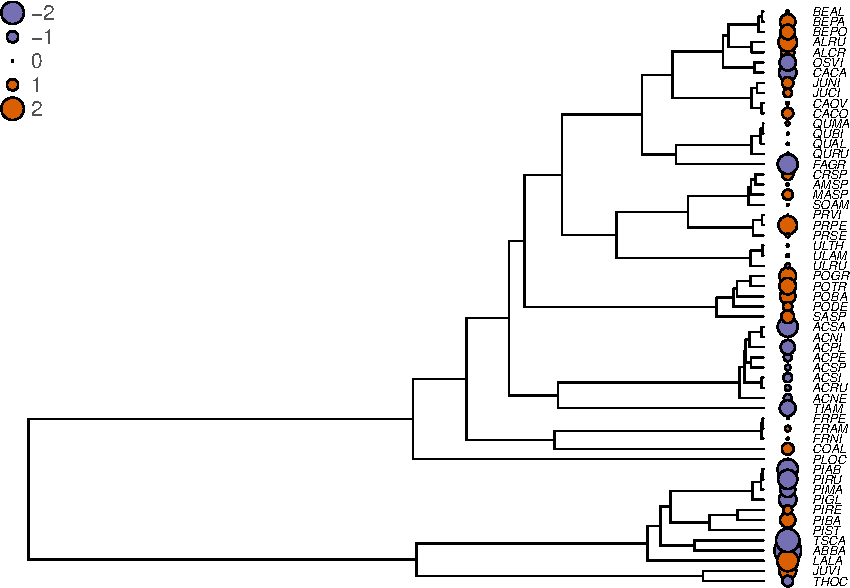
\includegraphics{pcm-workshop_files/figure-latex/Residuals of lm on phylogeny-1} \end{center}

\begin{Shaded}
\begin{Highlighting}[]
\CommentTok{\# Reset graphical parameters to defaults}
\FunctionTok{par}\NormalTok{(op) }
\end{Highlighting}
\end{Shaded}

You can see that in several cases, closely related species tend to have similar residuals (they are of the same color, which means that they are of the same side of the regression slope). This is problematic. Indeed, it shows that the assumption of independence of the ordinary least squares (OLS) regression no longer holds and the statistical tests for the null hypotheses are no longer valid. We will see next how phylogenetic generalized least squares can correct this.

\section{Challenge 1}\label{challenge-1}

In the \texttt{seedplantsdata} data frame, there were many different traits. Try to fit a regression of tree shade tolerance (\texttt{shade}) on the seed mass (\texttt{Sm}). In other words, test if shade tolerance can be explained by the seed mass of the trees. Then, try to see if the residuals are phylogenetically correlated.

\chapter{Phylogenetic generalized least squares (PGLS)}\label{pgls}

\section{Theory}\label{theory-1}

Phylogenetic generalized least squares (PGLS) is just a specific application of the broader method called generalized least squares (GLS). Generalized least squares relax the assumption that the error of the linear model has to be uncorrelated. They allow the user to specify the structure of that residual correlation. This is used, for instance, to correct for spatial correlation, time series, or phylogenetic correlation.

GLS have the same structure as Ordinary Least Squares (OLS):

\[\textbf{y} = \alpha + \beta \textbf{x} + \textbf{e}\]

The only difference is that the residuals are correlated with each other according to a correlation structure \(\textbf{C}\):

\[\textbf{e} \sim N(0,\sigma^2\textbf{C})\]

Here, \(\textbf{C}\) is a correlation matrix that describes how the residuals are correlated with each other. To be able to account for phylogenetic relationships in a PGLS, we thus need to be able to express the phylogenetic relationships in the form of a correlation matrix.

\subsection{Phylogenetic correlation structure}\label{phylogenetic-correlation-structure}

Phylogenetic relationships can be described using a correlation structure. Below, you have phylogenetic tree with branch lengths indicated above the branches.

\begin{flushleft}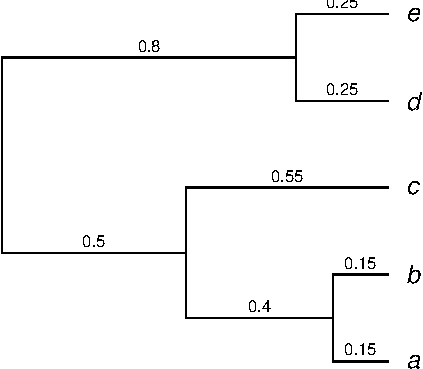
\includegraphics{pcm-workshop_files/figure-latex/phylogenetic tree example-1} \end{flushleft}

Now, this tree can be perfectly represented by a variance-covariance matrix.

\begin{verbatim}
##      a    b    c    d    e
## a 1.05 0.90 0.50 0.00 0.00
## b 0.90 1.05 0.50 0.00 0.00
## c 0.50 0.50 1.05 0.00 0.00
## d 0.00 0.00 0.00 1.05 0.80
## e 0.00 0.00 0.00 0.80 1.05
\end{verbatim}

The diagonal elements of the matrix are the species variances; these numbers represent the total distance from the root of the tree to the tips. It determines how much the tips have evolved from the root. The off-diagonal elements are the covariances between the species. They indicate the proportion of the time that the species have evolved together. This corresponds to the length of the branches that two species share, starting from the root of the tree. For instance, species \(a\) and \(c\) have shared a common history for 0.5 units of time; hence they have a covariance of 0.5. The greater the covariance, the longer the two species have shared the same evolutionary history.

If all the variation among species was due to phylogeny and none to selection, then this variance-covariance matrix would represent the expectation of how much all species would be similar to the other species.

\begin{quote}
Note that all the tips are equidistant from the root. When trees have this property, they are said to be \textbf{\emph{ultrametric}}. Most phylogenetic comparative methods require the trees to be ultrametric, although there are sometimes ways to relax this assumption. If you do not have an ultrametric tree, it is possible to make it ultrametric using the function \texttt{chronopl} of the \texttt{ape} package. But ideally, it is better to use a phylogenetic method that directly reconstruct ultrametric trees.
\end{quote}

The variance-covariance matrix of a phylogenetic tree can be obtained from a tree using the function \texttt{vcv} from the \texttt{ape} package.

\begin{Shaded}
\begin{Highlighting}[]
\CommentTok{\# \textquotesingle{}atree\textquotesingle{} corresponds to the phylogenetic tree shown above in newick format}
\NormalTok{atree }\OtherTok{\textless{}{-}} \StringTok{"(((a:0.15,b:0.15):0.4,c:0.55):0.5,(d:0.25,e:0.25):0.8);"}
\CommentTok{\# Let\textquotesingle{}s now read this tree and store it as a phylogenetic tree object in R}
\NormalTok{atree }\OtherTok{\textless{}{-}} \FunctionTok{read.tree}\NormalTok{(}\AttributeTok{text=}\NormalTok{atree)}
\CommentTok{\# Show the tree}
\FunctionTok{plot}\NormalTok{(atree)}
\end{Highlighting}
\end{Shaded}

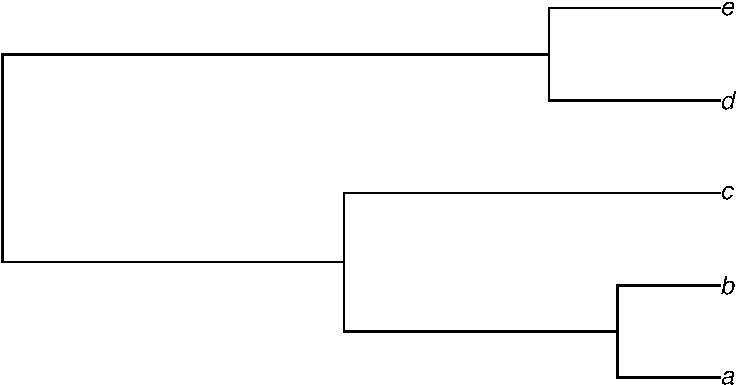
\includegraphics{pcm-workshop_files/figure-latex/vcv function-1.pdf}

\begin{Shaded}
\begin{Highlighting}[]
\CommentTok{\# Extract the variance{-}covariance matrix}
\NormalTok{varcovar }\OtherTok{\textless{}{-}} \FunctionTok{vcv}\NormalTok{(atree)}
\CommentTok{\# Print the variance{-}covariance matrix}
\NormalTok{varcovar}
\end{Highlighting}
\end{Shaded}

\begin{verbatim}
##      a    b    c    d    e
## a 1.05 0.90 0.50 0.00 0.00
## b 0.90 1.05 0.50 0.00 0.00
## c 0.50 0.50 1.05 0.00 0.00
## d 0.00 0.00 0.00 1.05 0.80
## e 0.00 0.00 0.00 0.80 1.05
\end{verbatim}

This is great, but we mentioned above that it is a correlation matric that we need in a GLS to account for the correlation in the residuals. To obtain a correlation matrix from the variance-covariance matrix shown above, you only need to divide the variance-covariance matrix by the length of the tree, or the distance from the root to the tips. It can also be obtained using the R function \texttt{cov2cor}.

\begin{Shaded}
\begin{Highlighting}[]
\CommentTok{\# Convert the covariance matrix to a correlation matrix}
\NormalTok{corrmat }\OtherTok{\textless{}{-}} \FunctionTok{cov2cor}\NormalTok{(varcovar)}
\CommentTok{\# Print the matrix, rounding the numbers to three decimals}
\FunctionTok{round}\NormalTok{(corrmat,}\DecValTok{3}\NormalTok{)}
\end{Highlighting}
\end{Shaded}

\begin{verbatim}
##       a     b     c     d     e
## a 1.000 0.857 0.476 0.000 0.000
## b 0.857 1.000 0.476 0.000 0.000
## c 0.476 0.476 1.000 0.000 0.000
## d 0.000 0.000 0.000 1.000 0.762
## e 0.000 0.000 0.000 0.762 1.000
\end{verbatim}

Now, the diagonal elements equal to 1, indicating that the species are perfectly correlated to themselves. Note that it is also possible to obtain directly the correlation matrix from the function \texttt{vcv} by using the \texttt{corr=TRUE} option.

\begin{Shaded}
\begin{Highlighting}[]
\CommentTok{\# Obtaining a correlation matrix using the \textquotesingle{}vcv\textquotesingle{} function}
\NormalTok{corrmat }\OtherTok{\textless{}{-}} \FunctionTok{vcv}\NormalTok{(atree,}\AttributeTok{corr=}\ConstantTok{TRUE}\NormalTok{)}
\FunctionTok{round}\NormalTok{(corrmat,}\DecValTok{3}\NormalTok{)}
\end{Highlighting}
\end{Shaded}

\begin{verbatim}
##       a     b     c     d     e
## a 1.000 0.857 0.476 0.000 0.000
## b 0.857 1.000 0.476 0.000 0.000
## c 0.476 0.476 1.000 0.000 0.000
## d 0.000 0.000 0.000 1.000 0.762
## e 0.000 0.000 0.000 0.762 1.000
\end{verbatim}

Now that we know how to obtain a correlation matrix from a phylogenetic tree, we are ready to run a PGLS.

\section{Challenge 2}\label{challenge-2}

Can you get the covariance matrix and the correlation matrix for the seed plants phylogenetic tree from the example above (\texttt{seedplantstree})?

\section{Practicals}\label{practicals}

There are several ways to run a PGLS in R. For instance, the package \texttt{caper} is a very well known package for PGLS. However, we will use the function \texttt{gls} here from the \texttt{nlme} package. This function is robust and has the advantage to be very flexible. Indeed, it allows to easily use more complex models such as mixed effect models, although this will not be discussed here.

Before we run the PGLS, let's run the basic model with the function \texttt{gls} as a reference. Running the standard linear model with the package \texttt{nlme} will allow to run model comparison functions in R (see below), which would not be possible is different models were fitted using different packages.

\begin{Shaded}
\begin{Highlighting}[]
\FunctionTok{require}\NormalTok{(nlme)}
\NormalTok{shade.pgls0 }\OtherTok{\textless{}{-}} \FunctionTok{gls}\NormalTok{(Shade }\SpecialCharTok{\textasciitilde{}}\NormalTok{ Wd, }\AttributeTok{data =}\NormalTok{ seedplantsdata)}
\FunctionTok{summary}\NormalTok{(shade.pgls0)}
\end{Highlighting}
\end{Shaded}

\begin{verbatim}
## Generalized least squares fit by REML
##   Model: Shade ~ Wd 
##   Data: seedplantsdata 
##       AIC     BIC    logLik
##   180.472 186.494 -87.23602
## 
## Coefficients:
##               Value Std.Error  t-value p-value
## (Intercept) 2.00098 0.7500707 2.667722  0.0100
## Wd          1.81296 1.5675668 1.156544  0.2525
## 
##  Correlation: 
##    (Intr)
## Wd -0.979
## 
## Standardized residuals:
##         Min          Q1         Med          Q3         Max 
## -1.63307700 -0.89457443  0.04911902  0.61207032  2.07940955 
## 
## Residual standard error: 1.145813 
## Degrees of freedom: 57 total; 55 residual
\end{verbatim}

You can see that the output is essentially identical to that of the \texttt{lm} function. However, there are some differences. One is the presence of the item ``Correlation:'' that gives the correlation among the estimated parameters. Also, the ``Standardized residuals'' are the raw residuals divided by the residual standard error (the raw residuals can be output with \texttt{residuals(shade.gls,"response")}).

Now, let's run a PGLS model. To assign the correlation matrix to the \texttt{gls} function, you simply need to use the \texttt{corr} option of the \texttt{gls} function. However, you need to use a specific correlation function so that R understands that it is a correlation matrix and estimate the model correctly.

There are several different types of correlation structures that are available in \texttt{R}. We will start by using one of the simplest one, called \texttt{corSymm}, that assumes that the correlation matrix is symmetric. This is the case with phylogenetic trees; the correlation between species \(a\) and \(b\) is the same as between \(b\) ad \(a\). Only the lower triangular part of the matrix has to be passed to the \texttt{corSymm} structure. If \texttt{mat} is the correlation matrix, this is done using the command \texttt{mat{[}lower.tri(mat){]}}. Then you pass the correlation matrix to \texttt{gls} using the \texttt{correlation} argument.

\begin{Shaded}
\begin{Highlighting}[]
\CommentTok{\# Calculate the correlation matrix from the tree}
\NormalTok{mat }\OtherTok{\textless{}{-}} \FunctionTok{vcv}\NormalTok{(seedplantstree,}\AttributeTok{corr=}\ConstantTok{TRUE}\NormalTok{)}
\CommentTok{\# Create the correlation structure for gls}
\NormalTok{corr.struct }\OtherTok{\textless{}{-}} \FunctionTok{corSymm}\NormalTok{(mat[}\FunctionTok{lower.tri}\NormalTok{(mat)],}\AttributeTok{fixed=}\ConstantTok{TRUE}\NormalTok{)}
\CommentTok{\# Run the pgls}
\NormalTok{shade.pgls1 }\OtherTok{\textless{}{-}} \FunctionTok{gls}\NormalTok{(Shade }\SpecialCharTok{\textasciitilde{}}\NormalTok{ Wd, }\AttributeTok{data =}\NormalTok{ seedplantsdata, }\AttributeTok{correlation=}\NormalTok{corr.struct)}
\FunctionTok{summary}\NormalTok{(shade.pgls1)}
\end{Highlighting}
\end{Shaded}

\begin{verbatim}
## Generalized least squares fit by REML
##   Model: Shade ~ Wd 
##   Data: seedplantsdata 
##        AIC      BIC    logLik
##   214.3762 220.3982 -104.1881
## 
## Correlation Structure: General
##  Formula: ~1 
##  Parameter estimate(s):
##  Correlation: 
##    1     2     3     4     5     6     7     8     9     10    11    12   
## 2  0.000                                                                  
## 3  0.000 0.967                                                            
## 4  0.000 0.967 0.976                                                      
## 5  0.000 0.967 0.981 0.976                                                
## 6  0.000 0.967 0.974 0.974 0.974                                          
## 7  0.000 0.967 0.997 0.976 0.981 0.974                                    
## 8  0.000 0.967 0.974 0.974 0.974 0.997 0.974                              
## 9  0.000 0.967 0.976 0.983 0.976 0.974 0.976 0.974                        
## 10 0.000 0.654 0.654 0.654 0.654 0.654 0.654 0.654 0.654                  
## 11 0.000 0.654 0.654 0.654 0.654 0.654 0.654 0.654 0.654 0.984            
## 12 0.000 0.654 0.654 0.654 0.654 0.654 0.654 0.654 0.654 0.726 0.726      
## 13 0.000 0.654 0.654 0.654 0.654 0.654 0.654 0.654 0.654 0.952 0.952 0.726
## 14 0.000 0.654 0.654 0.654 0.654 0.654 0.654 0.654 0.654 0.952 0.952 0.726
## 15 0.000 0.654 0.654 0.654 0.654 0.654 0.654 0.654 0.654 0.952 0.952 0.726
## 16 0.000 0.654 0.654 0.654 0.654 0.654 0.654 0.654 0.654 0.945 0.945 0.726
## 17 0.000 0.654 0.654 0.654 0.654 0.654 0.654 0.654 0.654 0.876 0.876 0.726
## 18 0.000 0.654 0.654 0.654 0.654 0.654 0.654 0.654 0.654 0.876 0.876 0.726
## 19 0.000 0.596 0.596 0.596 0.596 0.596 0.596 0.596 0.596 0.596 0.596 0.596
## 20 0.000 0.654 0.654 0.654 0.654 0.654 0.654 0.654 0.654 0.726 0.726 0.989
## 21 0.000 0.654 0.654 0.654 0.654 0.654 0.654 0.654 0.654 0.835 0.835 0.726
## 22 0.000 0.596 0.596 0.596 0.596 0.596 0.596 0.596 0.596 0.596 0.596 0.596
## 23 0.000 0.596 0.596 0.596 0.596 0.596 0.596 0.596 0.596 0.596 0.596 0.596
## 24 0.000 0.596 0.596 0.596 0.596 0.596 0.596 0.596 0.596 0.596 0.596 0.596
## 25 0.000 0.654 0.654 0.654 0.654 0.654 0.654 0.654 0.654 0.876 0.876 0.726
## 26 0.000 0.654 0.654 0.654 0.654 0.654 0.654 0.654 0.654 0.876 0.876 0.726
## 27 0.528 0.000 0.000 0.000 0.000 0.000 0.000 0.000 0.000 0.000 0.000 0.000
## 28 0.843 0.000 0.000 0.000 0.000 0.000 0.000 0.000 0.000 0.000 0.000 0.000
## 29 0.000 0.654 0.654 0.654 0.654 0.654 0.654 0.654 0.654 0.726 0.726 0.983
## 30 0.000 0.654 0.654 0.654 0.654 0.654 0.654 0.654 0.654 0.945 0.945 0.726
## 31 0.860 0.000 0.000 0.000 0.000 0.000 0.000 0.000 0.000 0.000 0.000 0.000
## 32 0.860 0.000 0.000 0.000 0.000 0.000 0.000 0.000 0.000 0.000 0.000 0.000
## 33 0.860 0.000 0.000 0.000 0.000 0.000 0.000 0.000 0.000 0.000 0.000 0.000
## 34 0.860 0.000 0.000 0.000 0.000 0.000 0.000 0.000 0.000 0.000 0.000 0.000
## 35 0.860 0.000 0.000 0.000 0.000 0.000 0.000 0.000 0.000 0.000 0.000 0.000
## 36 0.860 0.000 0.000 0.000 0.000 0.000 0.000 0.000 0.000 0.000 0.000 0.000
## 37 0.860 0.000 0.000 0.000 0.000 0.000 0.000 0.000 0.000 0.000 0.000 0.000
## 38 0.000 0.523 0.523 0.523 0.523 0.523 0.523 0.523 0.523 0.523 0.523 0.523
## 39 0.000 0.654 0.654 0.654 0.654 0.654 0.654 0.654 0.654 0.675 0.675 0.675
## 40 0.000 0.654 0.654 0.654 0.654 0.654 0.654 0.654 0.654 0.675 0.675 0.675
## 41 0.000 0.654 0.654 0.654 0.654 0.654 0.654 0.654 0.654 0.675 0.675 0.675
## 42 0.000 0.654 0.654 0.654 0.654 0.654 0.654 0.654 0.654 0.675 0.675 0.675
## 43 0.000 0.654 0.654 0.654 0.654 0.654 0.654 0.654 0.654 0.726 0.726 0.898
## 44 0.000 0.654 0.654 0.654 0.654 0.654 0.654 0.654 0.654 0.726 0.726 0.898
## 45 0.000 0.654 0.654 0.654 0.654 0.654 0.654 0.654 0.654 0.726 0.726 0.898
## 46 0.000 0.654 0.654 0.654 0.654 0.654 0.654 0.654 0.654 0.835 0.835 0.726
## 47 0.000 0.654 0.654 0.654 0.654 0.654 0.654 0.654 0.654 0.835 0.835 0.726
## 48 0.000 0.654 0.654 0.654 0.654 0.654 0.654 0.654 0.654 0.835 0.835 0.726
## 49 0.000 0.654 0.654 0.654 0.654 0.654 0.654 0.654 0.654 0.835 0.835 0.726
## 50 0.000 0.654 0.654 0.654 0.654 0.654 0.654 0.654 0.654 0.675 0.675 0.675
## 51 0.000 0.654 0.654 0.654 0.654 0.654 0.654 0.654 0.654 0.726 0.726 0.980
## 52 0.528 0.000 0.000 0.000 0.000 0.000 0.000 0.000 0.000 0.000 0.000 0.000
## 53 0.000 0.720 0.720 0.720 0.720 0.720 0.720 0.720 0.720 0.654 0.654 0.654
## 54 0.906 0.000 0.000 0.000 0.000 0.000 0.000 0.000 0.000 0.000 0.000 0.000
## 55 0.000 0.654 0.654 0.654 0.654 0.654 0.654 0.654 0.654 0.726 0.726 0.800
## 56 0.000 0.654 0.654 0.654 0.654 0.654 0.654 0.654 0.654 0.726 0.726 0.800
## 57 0.000 0.654 0.654 0.654 0.654 0.654 0.654 0.654 0.654 0.726 0.726 0.800
##    13    14    15    16    17    18    19    20    21    22    23    24   
## 2                                                                         
## 3                                                                         
## 4                                                                         
## 5                                                                         
## 6                                                                         
## 7                                                                         
## 8                                                                         
## 9                                                                         
## 10                                                                        
## 11                                                                        
## 12                                                                        
## 13                                                                        
## 14 0.998                                                                  
## 15 0.994 0.994                                                            
## 16 0.945 0.945 0.945                                                      
## 17 0.876 0.876 0.876 0.876                                                
## 18 0.876 0.876 0.876 0.876 0.998                                          
## 19 0.596 0.596 0.596 0.596 0.596 0.596                                    
## 20 0.726 0.726 0.726 0.726 0.726 0.726 0.596                              
## 21 0.835 0.835 0.835 0.835 0.835 0.835 0.596 0.726                        
## 22 0.596 0.596 0.596 0.596 0.596 0.596 0.715 0.596 0.596                  
## 23 0.596 0.596 0.596 0.596 0.596 0.596 0.715 0.596 0.596 0.997            
## 24 0.596 0.596 0.596 0.596 0.596 0.596 0.715 0.596 0.596 0.999 0.997      
## 25 0.876 0.876 0.876 0.876 0.984 0.984 0.596 0.726 0.835 0.596 0.596 0.596
## 26 0.876 0.876 0.876 0.876 0.984 0.984 0.596 0.726 0.835 0.596 0.596 0.596
## 27 0.000 0.000 0.000 0.000 0.000 0.000 0.000 0.000 0.000 0.000 0.000 0.000
## 28 0.000 0.000 0.000 0.000 0.000 0.000 0.000 0.000 0.000 0.000 0.000 0.000
## 29 0.726 0.726 0.726 0.726 0.726 0.726 0.596 0.983 0.726 0.596 0.596 0.596
## 30 0.945 0.945 0.945 0.988 0.876 0.876 0.596 0.726 0.835 0.596 0.596 0.596
## 31 0.000 0.000 0.000 0.000 0.000 0.000 0.000 0.000 0.000 0.000 0.000 0.000
## 32 0.000 0.000 0.000 0.000 0.000 0.000 0.000 0.000 0.000 0.000 0.000 0.000
## 33 0.000 0.000 0.000 0.000 0.000 0.000 0.000 0.000 0.000 0.000 0.000 0.000
## 34 0.000 0.000 0.000 0.000 0.000 0.000 0.000 0.000 0.000 0.000 0.000 0.000
## 35 0.000 0.000 0.000 0.000 0.000 0.000 0.000 0.000 0.000 0.000 0.000 0.000
## 36 0.000 0.000 0.000 0.000 0.000 0.000 0.000 0.000 0.000 0.000 0.000 0.000
## 37 0.000 0.000 0.000 0.000 0.000 0.000 0.000 0.000 0.000 0.000 0.000 0.000
## 38 0.523 0.523 0.523 0.523 0.523 0.523 0.523 0.523 0.523 0.523 0.523 0.523
## 39 0.675 0.675 0.675 0.675 0.675 0.675 0.596 0.675 0.675 0.596 0.596 0.596
## 40 0.675 0.675 0.675 0.675 0.675 0.675 0.596 0.675 0.675 0.596 0.596 0.596
## 41 0.675 0.675 0.675 0.675 0.675 0.675 0.596 0.675 0.675 0.596 0.596 0.596
## 42 0.675 0.675 0.675 0.675 0.675 0.675 0.596 0.675 0.675 0.596 0.596 0.596
## 43 0.726 0.726 0.726 0.726 0.726 0.726 0.596 0.898 0.726 0.596 0.596 0.596
## 44 0.726 0.726 0.726 0.726 0.726 0.726 0.596 0.898 0.726 0.596 0.596 0.596
## 45 0.726 0.726 0.726 0.726 0.726 0.726 0.596 0.898 0.726 0.596 0.596 0.596
## 46 0.835 0.835 0.835 0.835 0.835 0.835 0.596 0.726 0.881 0.596 0.596 0.596
## 47 0.835 0.835 0.835 0.835 0.835 0.835 0.596 0.726 0.881 0.596 0.596 0.596
## 48 0.835 0.835 0.835 0.835 0.835 0.835 0.596 0.726 0.881 0.596 0.596 0.596
## 49 0.835 0.835 0.835 0.835 0.835 0.835 0.596 0.726 0.881 0.596 0.596 0.596
## 50 0.675 0.675 0.675 0.675 0.675 0.675 0.596 0.675 0.675 0.596 0.596 0.596
## 51 0.726 0.726 0.726 0.726 0.726 0.726 0.596 0.980 0.726 0.596 0.596 0.596
## 52 0.000 0.000 0.000 0.000 0.000 0.000 0.000 0.000 0.000 0.000 0.000 0.000
## 53 0.654 0.654 0.654 0.654 0.654 0.654 0.596 0.654 0.654 0.596 0.596 0.596
## 54 0.000 0.000 0.000 0.000 0.000 0.000 0.000 0.000 0.000 0.000 0.000 0.000
## 55 0.726 0.726 0.726 0.726 0.726 0.726 0.596 0.800 0.726 0.596 0.596 0.596
## 56 0.726 0.726 0.726 0.726 0.726 0.726 0.596 0.800 0.726 0.596 0.596 0.596
## 57 0.726 0.726 0.726 0.726 0.726 0.726 0.596 0.800 0.726 0.596 0.596 0.596
##    25    26    27    28    29    30    31    32    33    34    35    36   
## 2                                                                         
## 3                                                                         
## 4                                                                         
## 5                                                                         
## 6                                                                         
## 7                                                                         
## 8                                                                         
## 9                                                                         
## 10                                                                        
## 11                                                                        
## 12                                                                        
## 13                                                                        
## 14                                                                        
## 15                                                                        
## 16                                                                        
## 17                                                                        
## 18                                                                        
## 19                                                                        
## 20                                                                        
## 21                                                                        
## 22                                                                        
## 23                                                                        
## 24                                                                        
## 25                                                                        
## 26 0.992                                                                  
## 27 0.000 0.000                                                            
## 28 0.000 0.000 0.528                                                      
## 29 0.726 0.726 0.000 0.000                                                
## 30 0.876 0.876 0.000 0.000 0.726                                          
## 31 0.000 0.000 0.528 0.843 0.000 0.000                                    
## 32 0.000 0.000 0.528 0.843 0.000 0.000 0.874                              
## 33 0.000 0.000 0.528 0.843 0.000 0.000 0.985 0.874                        
## 34 0.000 0.000 0.528 0.843 0.000 0.000 0.997 0.874 0.985                  
## 35 0.000 0.000 0.528 0.843 0.000 0.000 0.874 0.965 0.874 0.874            
## 36 0.000 0.000 0.528 0.843 0.000 0.000 0.999 0.874 0.985 0.997 0.874      
## 37 0.000 0.000 0.528 0.843 0.000 0.000 0.874 0.926 0.874 0.874 0.926 0.874
## 38 0.523 0.523 0.000 0.000 0.523 0.523 0.000 0.000 0.000 0.000 0.000 0.000
## 39 0.675 0.675 0.000 0.000 0.675 0.675 0.000 0.000 0.000 0.000 0.000 0.000
## 40 0.675 0.675 0.000 0.000 0.675 0.675 0.000 0.000 0.000 0.000 0.000 0.000
## 41 0.675 0.675 0.000 0.000 0.675 0.675 0.000 0.000 0.000 0.000 0.000 0.000
## 42 0.675 0.675 0.000 0.000 0.675 0.675 0.000 0.000 0.000 0.000 0.000 0.000
## 43 0.726 0.726 0.000 0.000 0.898 0.726 0.000 0.000 0.000 0.000 0.000 0.000
## 44 0.726 0.726 0.000 0.000 0.898 0.726 0.000 0.000 0.000 0.000 0.000 0.000
## 45 0.726 0.726 0.000 0.000 0.898 0.726 0.000 0.000 0.000 0.000 0.000 0.000
## 46 0.835 0.835 0.000 0.000 0.726 0.835 0.000 0.000 0.000 0.000 0.000 0.000
## 47 0.835 0.835 0.000 0.000 0.726 0.835 0.000 0.000 0.000 0.000 0.000 0.000
## 48 0.835 0.835 0.000 0.000 0.726 0.835 0.000 0.000 0.000 0.000 0.000 0.000
## 49 0.835 0.835 0.000 0.000 0.726 0.835 0.000 0.000 0.000 0.000 0.000 0.000
## 50 0.675 0.675 0.000 0.000 0.675 0.675 0.000 0.000 0.000 0.000 0.000 0.000
## 51 0.726 0.726 0.000 0.000 0.980 0.726 0.000 0.000 0.000 0.000 0.000 0.000
## 52 0.000 0.000 0.918 0.528 0.000 0.000 0.528 0.528 0.528 0.528 0.528 0.528
## 53 0.654 0.654 0.000 0.000 0.654 0.654 0.000 0.000 0.000 0.000 0.000 0.000
## 54 0.000 0.000 0.528 0.843 0.000 0.000 0.860 0.860 0.860 0.860 0.860 0.860
## 55 0.726 0.726 0.000 0.000 0.800 0.726 0.000 0.000 0.000 0.000 0.000 0.000
## 56 0.726 0.726 0.000 0.000 0.800 0.726 0.000 0.000 0.000 0.000 0.000 0.000
## 57 0.726 0.726 0.000 0.000 0.800 0.726 0.000 0.000 0.000 0.000 0.000 0.000
##    37    38    39    40    41    42    43    44    45    46    47    48   
## 2                                                                         
## 3                                                                         
## 4                                                                         
## 5                                                                         
## 6                                                                         
## 7                                                                         
## 8                                                                         
## 9                                                                         
## 10                                                                        
## 11                                                                        
## 12                                                                        
## 13                                                                        
## 14                                                                        
## 15                                                                        
## 16                                                                        
## 17                                                                        
## 18                                                                        
## 19                                                                        
## 20                                                                        
## 21                                                                        
## 22                                                                        
## 23                                                                        
## 24                                                                        
## 25                                                                        
## 26                                                                        
## 27                                                                        
## 28                                                                        
## 29                                                                        
## 30                                                                        
## 31                                                                        
## 32                                                                        
## 33                                                                        
## 34                                                                        
## 35                                                                        
## 36                                                                        
## 37                                                                        
## 38 0.000                                                                  
## 39 0.000 0.523                                                            
## 40 0.000 0.523 0.959                                                      
## 41 0.000 0.523 0.964 0.959                                                
## 42 0.000 0.523 0.964 0.959 0.982                                          
## 43 0.000 0.523 0.675 0.675 0.675 0.675                                    
## 44 0.000 0.523 0.675 0.675 0.675 0.675 0.986                              
## 45 0.000 0.523 0.675 0.675 0.675 0.675 0.998 0.986                        
## 46 0.000 0.523 0.675 0.675 0.675 0.675 0.726 0.726 0.726                  
## 47 0.000 0.523 0.675 0.675 0.675 0.675 0.726 0.726 0.726 0.997            
## 48 0.000 0.523 0.675 0.675 0.675 0.675 0.726 0.726 0.726 0.997 0.999      
## 49 0.000 0.523 0.675 0.675 0.675 0.675 0.726 0.726 0.726 0.984 0.984 0.984
## 50 0.000 0.523 0.936 0.936 0.936 0.936 0.675 0.675 0.675 0.675 0.675 0.675
## 51 0.000 0.523 0.675 0.675 0.675 0.675 0.898 0.898 0.898 0.726 0.726 0.726
## 52 0.528 0.000 0.000 0.000 0.000 0.000 0.000 0.000 0.000 0.000 0.000 0.000
## 53 0.000 0.523 0.654 0.654 0.654 0.654 0.654 0.654 0.654 0.654 0.654 0.654
## 54 0.860 0.000 0.000 0.000 0.000 0.000 0.000 0.000 0.000 0.000 0.000 0.000
## 55 0.000 0.523 0.675 0.675 0.675 0.675 0.800 0.800 0.800 0.726 0.726 0.726
## 56 0.000 0.523 0.675 0.675 0.675 0.675 0.800 0.800 0.800 0.726 0.726 0.726
## 57 0.000 0.523 0.675 0.675 0.675 0.675 0.800 0.800 0.800 0.726 0.726 0.726
##    49    50    51    52    53    54    55    56   
## 2                                                 
## 3                                                 
## 4                                                 
## 5                                                 
## 6                                                 
## 7                                                 
## 8                                                 
## 9                                                 
## 10                                                
## 11                                                
## 12                                                
## 13                                                
## 14                                                
## 15                                                
## 16                                                
## 17                                                
## 18                                                
## 19                                                
## 20                                                
## 21                                                
## 22                                                
## 23                                                
## 24                                                
## 25                                                
## 26                                                
## 27                                                
## 28                                                
## 29                                                
## 30                                                
## 31                                                
## 32                                                
## 33                                                
## 34                                                
## 35                                                
## 36                                                
## 37                                                
## 38                                                
## 39                                                
## 40                                                
## 41                                                
## 42                                                
## 43                                                
## 44                                                
## 45                                                
## 46                                                
## 47                                                
## 48                                                
## 49                                                
## 50 0.675                                          
## 51 0.726 0.675                                    
## 52 0.000 0.000 0.000                              
## 53 0.654 0.654 0.654 0.000                        
## 54 0.000 0.000 0.000 0.528 0.000                  
## 55 0.726 0.675 0.800 0.000 0.654 0.000            
## 56 0.726 0.675 0.800 0.000 0.654 0.000 0.983      
## 57 0.726 0.675 0.800 0.000 0.654 0.000 0.999 0.983
## 
## Coefficients:
##                Value Std.Error   t-value p-value
## (Intercept) 0.911433  4.409058 0.2067184  0.8370
## Wd          4.361028  1.693349 2.5753865  0.0127
## 
##  Correlation: 
##    (Intr)
## Wd -0.166
## 
## Standardized residuals:
##         Min          Q1         Med          Q3         Max 
## -0.26890642 -0.16431866 -0.02645422  0.09638984  0.34953444 
## 
## Residual standard error: 7.455109 
## Degrees of freedom: 57 total; 55 residual
\end{verbatim}

Note that the term \texttt{fixed=TRUE} in the corSymm structure indicates that the correlation structure is fixed during the parameter optimization.

The output is similar to that of the model without the correlation, except for the output of the correlation matrix.

Interestingly, you can see that the coefficient estimate for the slope is greater (4.361) than with standard regression and also significant (\(p\)=0.0127). This is a positive example of PGLS. Indeed, the relationship between shade tolerance and wood density was obscured by the phylogenetic correlation of the residuals. Once this correlation is accounted for, the significant relationship is revealed.

A significant relationship between shade tolerance and wood density actually make sense, even though this relationship is most likely not causal. Indeed, shade tolerant trees are generally sucessional species and often grow slower, partly because of the limited light availability, and thus tend to develop higher density woods.

Now, let's have a look at the residuals of the model. To extract residuals corrected by the correlation structure, you need to ask for the normalized residuals.

\begin{Shaded}
\begin{Highlighting}[]
\CommentTok{\# Extract the residuals corrected by the correlation structure}
\NormalTok{pgls1.res }\OtherTok{\textless{}{-}} \FunctionTok{residuals}\NormalTok{(shade.pgls1,}\AttributeTok{type=}\StringTok{"normalized"}\NormalTok{)}
\CommentTok{\# Change the graphical parameters}
\NormalTok{op }\OtherTok{\textless{}{-}} \FunctionTok{par}\NormalTok{(}\AttributeTok{mar=}\FunctionTok{c}\NormalTok{(}\DecValTok{1}\NormalTok{,}\DecValTok{1}\NormalTok{,}\DecValTok{1}\NormalTok{,}\DecValTok{1}\NormalTok{))}
\CommentTok{\# Same plotting as above except for using pgls1.res as residuals}
\FunctionTok{plot}\NormalTok{(seedplantstree,}\AttributeTok{type=}\StringTok{"p"}\NormalTok{,}\ConstantTok{TRUE}\NormalTok{,}\AttributeTok{label.offset=}\FloatTok{0.01}\NormalTok{,}\AttributeTok{cex=}\FloatTok{0.5}\NormalTok{,}\AttributeTok{no.margin=}\ConstantTok{FALSE}\NormalTok{)}
\FunctionTok{tiplabels}\NormalTok{(}\AttributeTok{pch=}\DecValTok{21}\NormalTok{,}\AttributeTok{bg=}\NormalTok{cols[}\FunctionTok{ifelse}\NormalTok{(pgls1.res}\SpecialCharTok{\textgreater{}}\DecValTok{0}\NormalTok{,}\DecValTok{1}\NormalTok{,}\DecValTok{2}\NormalTok{)],}\AttributeTok{col=}\StringTok{"black"}\NormalTok{,}
          \AttributeTok{cex=}\FunctionTok{abs}\NormalTok{(pgls1.res),}\AttributeTok{adj=}\FloatTok{0.505}\NormalTok{)}
\FunctionTok{legend}\NormalTok{(}\StringTok{"topleft"}\NormalTok{,}\AttributeTok{legend=}\FunctionTok{c}\NormalTok{(}\StringTok{"{-}2"}\NormalTok{,}\StringTok{"{-}1"}\NormalTok{,}\StringTok{"0"}\NormalTok{,}\StringTok{"1"}\NormalTok{,}\StringTok{"2"}\NormalTok{),}\AttributeTok{pch=}\DecValTok{21}\NormalTok{,}
       \AttributeTok{pt.bg=}\NormalTok{cols[}\FunctionTok{c}\NormalTok{(}\DecValTok{1}\NormalTok{,}\DecValTok{1}\NormalTok{,}\DecValTok{1}\NormalTok{,}\DecValTok{2}\NormalTok{,}\DecValTok{2}\NormalTok{)],}\AttributeTok{bty=}\StringTok{"n"}\NormalTok{,}
       \AttributeTok{text.col=}\StringTok{"black"}\NormalTok{,}\AttributeTok{cex=}\FloatTok{0.8}\NormalTok{,}\AttributeTok{pt.cex=}\FunctionTok{c}\NormalTok{(}\DecValTok{2}\NormalTok{,}\DecValTok{1}\NormalTok{,}\FloatTok{0.1}\NormalTok{,}\DecValTok{1}\NormalTok{,}\DecValTok{2}\NormalTok{))}
\end{Highlighting}
\end{Shaded}

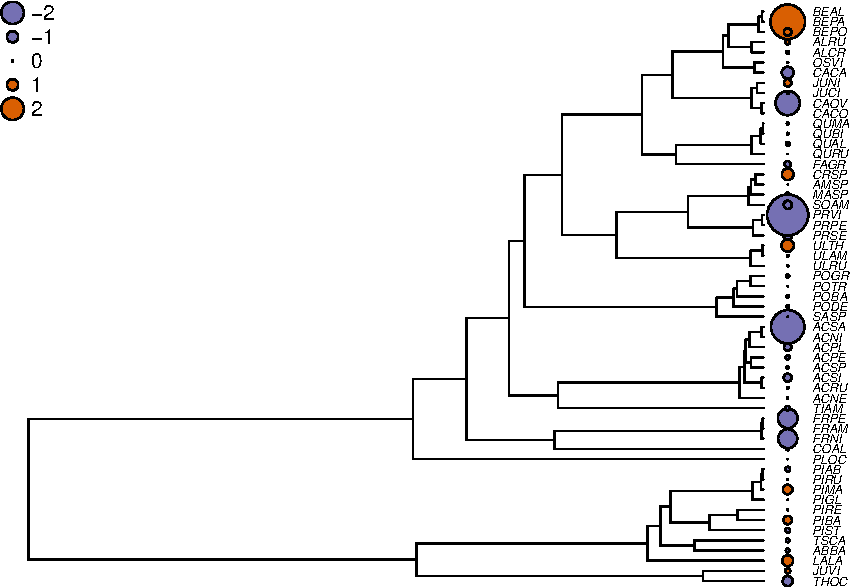
\includegraphics{pcm-workshop_files/figure-latex/pgls residual fit-1.pdf}

\begin{Shaded}
\begin{Highlighting}[]
\CommentTok{\# Reset graphical parameters to defaults}
\FunctionTok{par}\NormalTok{(op) }
\end{Highlighting}
\end{Shaded}

If you compare with the ordinary least squares optimization, the residuals are much less phylogenetically correlated.

\subsection{Other correlation structures}\label{other-correlation-structures}

In the previous PGLS, we have used the corSymm structure to pass the phylogenetic correlation structure to the gls. This is perfectly fine, but there are more simple ways. Julien Dutheil has developped phylogenetic structures to be used especially in PGLS.

The one we used above is equivalent to the \texttt{corBrownian} structure of \texttt{ape}. This approach is easier and you just have to pass the tree to the correlation structure. Here is the same example using the \texttt{corBrownian} structure.

\begin{Shaded}
\begin{Highlighting}[]
\CommentTok{\# Get the correlation structure}
\NormalTok{bm.corr }\OtherTok{\textless{}{-}} \FunctionTok{corBrownian}\NormalTok{(}\AttributeTok{phy=}\NormalTok{seedplantstree, }\AttributeTok{form=}\SpecialCharTok{\textasciitilde{}}\NormalTok{Code)}
\CommentTok{\# PGLS}
\NormalTok{shade.pgls1b }\OtherTok{\textless{}{-}} \FunctionTok{gls}\NormalTok{(Shade }\SpecialCharTok{\textasciitilde{}}\NormalTok{ Wd, }\AttributeTok{data =}\NormalTok{ seedplantsdata, }\AttributeTok{correlation=}\NormalTok{bm.corr)}
\FunctionTok{summary}\NormalTok{(shade.pgls1b)}
\end{Highlighting}
\end{Shaded}

\begin{verbatim}
## Generalized least squares fit by REML
##   Model: Shade ~ Wd 
##   Data: seedplantsdata 
##        AIC      BIC    logLik
##   214.3762 220.3982 -104.1881
## 
## Correlation Structure: corBrownian
##  Formula: ~Code 
##  Parameter estimate(s):
## numeric(0)
## 
## Coefficients:
##                Value Std.Error   t-value p-value
## (Intercept) 0.911433  4.409058 0.2067184  0.8370
## Wd          4.361028  1.693349 2.5753865  0.0127
## 
##  Correlation: 
##    (Intr)
## Wd -0.166
## 
## Standardized residuals:
##         Min          Q1         Med          Q3         Max 
## -0.26890642 -0.16431866 -0.02645422  0.09638984  0.34953444 
## 
## Residual standard error: 7.455109 
## Degrees of freedom: 57 total; 55 residual
\end{verbatim}

You can see that the results are identical. The only difference is that the correlation structure is not outputed in the summary. The \texttt{numeric(0)} means that no parameter was estimated during the optimization (it is fixed).

Now, you might wonder why the correlation structure is called corBrownian. This is because is uses Brownian motion to model the evolution along the branch of the tree. This is often refferred as a neutral model. If you want to know more about the Brownian Motion model, you can look at the section \ref{BM-model} on this model.

\section{Challenge 3}\label{challenge-3}

Fit a PGLS model to see whether the seed mass (\texttt{Sm}) explains shade tolerance (\texttt{Shade}) with the seedplantdataset. How does it compare to the results from the standard regression.

\chapter{Phylogenetic Independent Contrasts}\label{pic}

Let's make a digression to look at Phylogenetic Independent Contrasts (PIC). PIC were the first comparative approach proposed to deal with phylogenetic non independence \citep{felsenstein1985phylogenies}. Although they are less flexible than PGLS, they give the same results. Let's see how they can be used.

Phylogenetic independent contrast are estimated one trait at a time. They essentially transform the observed trait in contrasts that are not correlated with the phylogeny. This can be done in R using the \texttt{pic} function of the \texttt{ape} package.

\begin{Shaded}
\begin{Highlighting}[]
\CommentTok{\# Estimate PIC for shade tolerance }
\NormalTok{Shade.pic }\OtherTok{\textless{}{-}} \FunctionTok{pic}\NormalTok{(seedplantsdata}\SpecialCharTok{$}\NormalTok{Shade, }\AttributeTok{phy=}\NormalTok{seedplantstree)}
\CommentTok{\# Estimate PIC for Wood density }
\NormalTok{Wd.pic }\OtherTok{\textless{}{-}} \FunctionTok{pic}\NormalTok{(seedplantsdata}\SpecialCharTok{$}\NormalTok{Wd, }\AttributeTok{phy=}\NormalTok{seedplantstree)}
\end{Highlighting}
\end{Shaded}

Once this is done, the only thing to do is to fit a regression between these contrast. Note that it is important that the intercept is fixed to 0 in the model. This is done by adding \texttt{-\ 1} to the right of the formula.

\begin{Shaded}
\begin{Highlighting}[]
\CommentTok{\# Estimate PIC for shade tolerance}
\NormalTok{pic.results }\OtherTok{\textless{}{-}} \FunctionTok{lm}\NormalTok{(Shade.pic }\SpecialCharTok{\textasciitilde{}}\NormalTok{ Wd.pic }\SpecialCharTok{{-}} \DecValTok{1}\NormalTok{)}
\FunctionTok{summary}\NormalTok{(pic.results)}
\end{Highlighting}
\end{Shaded}

\begin{verbatim}
## 
## Call:
## lm(formula = Shade.pic ~ Wd.pic - 1)
## 
## Residuals:
##     Min      1Q  Median      3Q     Max 
## -71.943  -4.106   1.013   5.679  21.614 
## 
## Coefficients:
##        Estimate Std. Error t value Pr(>|t|)  
## Wd.pic    4.361      1.693   2.575   0.0127 *
## ---
## Signif. codes:  0 '***' 0.001 '**' 0.01 '*' 0.05 '.' 0.1 ' ' 1
## 
## Residual standard error: 19.21 on 55 degrees of freedom
## Multiple R-squared:  0.1076, Adjusted R-squared:  0.09139 
## F-statistic: 6.633 on 1 and 55 DF,  p-value: 0.01273
\end{verbatim}

You can see that the slope estimate, \texttt{4.361}, it identical to the slope estimate obtained with PGLS. Same thing for the p-value. The main retriction with PIC is that you are limited in always comparing two variables. Much more flexibility is possible with PGLS.

\chapter{Relaxing the assumption that residuals need to be perfectly phylogenetically correlated}\label{relaxing-the-assumption-that-residuals-need-to-be-perfectly-phylogenetically-correlated}

Phylogenetic Generalized Least Squares assume that the residuals are perfectly phylogenetically correlated. This is relatively constraining because it means that other sources of errors that are not phylogenetically correlated are not allowed by the model. Moreover, if these exist, they can bias the results of the PGLS \citep{revell2010phylogenetic}.

There are ways to relax this assumption, and one of this is to use a type of correlation structure that allows to relax this assumption.

\section{Theory: Pagel's correlation structure}\label{theory-pagels-correlation-structure}

When controling for phylogenetic relationships with phylogenetic generalized least squares, we assume that the residuals are perfectly correlated according to the correlation structure. In practice, it might not be always the case and it is difficult to really know how important it is to control for the phylogenetic relationship in a specific case. For instance, for a given study, the correlation in the residuals might not be highly phylogenetically correlated.

This is possible to account for this using the \(\lambda\) model of Pagel \citep{pagel1999inferring}. The idea is to multiply the off-diagonal of the correlation matrix (essentially the branch lengths of the phylogeny) by a parameter \(\lambda\), but not the diagonal values. This essentially leads to a modification of branch lengths of the phylogeny. A \(\lambda\) value near zero gives very shorts internal branches and long tip branches. This, in effect, reduces the phylogenetic correlations (the effect of the phylogeny is reduced). At the opposite, if \(\lambda\) is close to 1, then the modified phylogeny resembles the true phylogeny. Indeed, the parameter \(\lambda\) is often interpreted as a parameter of phylogenetic signal; as such, a greater \(\lambda\) value implies a stronger phylogenetic signal.

The following figure shows how different lambda values affect the shape of the Quebec trees phylogeny.

\begin{center}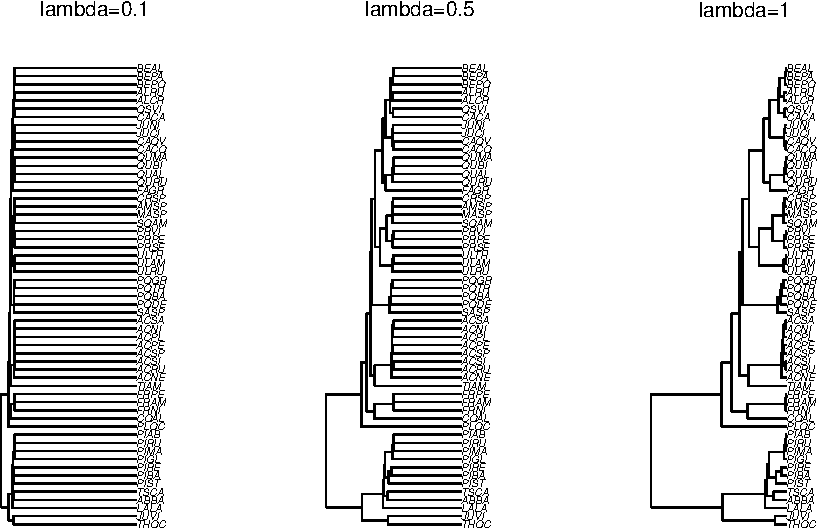
\includegraphics{pcm-workshop_files/figure-latex/alpha example-1} \end{center}

You can see that with small values of lambda, the weight given to the shared history (the phylogeny) are greatly reduced. The long terminal branches somewhat indicates that there could be a lot more variation in the residuals that are independent of the other species. This variation could be due to other factors that are included in the estimates of each species but that are independent of the phylogeny (such as measurement errors for instance).

\section{Practicals}\label{practicals-1}

Pagel's \(\lambda\) model can be used in PGLS using the \texttt{corPagel} correlation structure. The usage of this correlation structure is similar to that of the \texttt{corBrownian} structure, except that you need to provide a starting parameter value for \(\lambda\).

\begin{Shaded}
\begin{Highlighting}[]
\CommentTok{\# Get the correlation structure}
\NormalTok{pagel.corr }\OtherTok{\textless{}{-}} \FunctionTok{corPagel}\NormalTok{(}\FloatTok{0.3}\NormalTok{, }\AttributeTok{phy=}\NormalTok{seedplantstree, }\AttributeTok{fixed=}\ConstantTok{FALSE}\NormalTok{, }\AttributeTok{form=}\SpecialCharTok{\textasciitilde{}}\NormalTok{Code)}
\end{Highlighting}
\end{Shaded}

The value given to \texttt{corPagel} is the starting value for the \(\lambda\) parameter. Also, note that the option \texttt{fixed=} is set to \texttt{FALSE} This means that the \(\lambda\) parameter will be optimized using generalized least squares. If it was set to \texttt{TRUE}, then the model would be fitted with the starting parameter, here \texttt{0.3}. The \texttt{form=\textasciitilde{}Code} points to the column \texttt{Code} of the dataset for ordering the tree in the same order as the dataframe when fitting the function.

Let's now fit the PGLS with this correlation structure.

\begin{Shaded}
\begin{Highlighting}[]
\CommentTok{\# PGLS with coraPagel}
\NormalTok{shade.pgls2 }\OtherTok{\textless{}{-}} \FunctionTok{gls}\NormalTok{(Shade }\SpecialCharTok{\textasciitilde{}}\NormalTok{ Wd, }\AttributeTok{data =}\NormalTok{ seedplantsdata, }\AttributeTok{correlation=}\NormalTok{pagel.corr)}
\FunctionTok{summary}\NormalTok{(shade.pgls2)}
\end{Highlighting}
\end{Shaded}

\begin{verbatim}
## Generalized least squares fit by REML
##   Model: Shade ~ Wd 
##   Data: seedplantsdata 
##        AIC     BIC    logLik
##   163.3967 171.426 -77.69833
## 
## Correlation Structure: corPagel
##  Formula: ~Code 
##  Parameter estimate(s):
##    lambda 
## 0.9581665 
## 
## Coefficients:
##                Value Std.Error   t-value p-value
## (Intercept) 1.254987  1.636575 0.7668377  0.4465
## Wd          3.573527  1.497808 2.3858381  0.0205
## 
##  Correlation: 
##    (Intr)
## Wd -0.397
## 
## Standardized residuals:
##         Min          Q1         Med          Q3         Max 
## -0.75145692 -0.44908843 -0.05417524  0.25655008  0.96493685 
## 
## Residual standard error: 2.621947 
## Degrees of freedom: 57 total; 55 residual
\end{verbatim}

You can see that gls has estimated the \(\lambda\) parameter, which is 0.958 here. Because the estimated \(\lambda\) is very close to 1, we can conclude that residuals of the model were strongly phylogenetically correlated. This, in turns, thus confirms the importance of using a PGLS with this model. If the \(\lambda\) estimated would have been close to 0, it would have suggested that the PGLS is not necessary. Note, however, that using this approach assures you to never obtained a biased statistical result. Actually, I \textbf{strongly recommend} that you always use this correlation structure in your statistical analyses.

\section{Challenge 4}\label{challenge-4}

Try to fit a PGLS with a Pagel correlation structure when regressing Shade tolerance on seed mass. Are the residuals as phylogenetically correlated than in the previous regression with wood density?

\section{Other correlation structures (or evolutionary models)}\label{other-correlation-structures-or-evolutionary-models}

The correlation structures available in the package \texttt{ape} offer other alternatives for the assumed model of character evolution. For instance, the \texttt{corMartins} correlation structure models selection using the Ornstein-Uhlenbeck (or Hansen) model with parameter \(\alpha\) that determines the strength of the selection. Also, \texttt{corBlomberg} models accelerating or decelerating Brownian evolution, that is, the evolutionary rate of the Brownian motion is either accelerating or decelerating with time with this model. It is possible to do model comparisons to decide which model best fit the residual variation.

\chapter{Phylogenetic ANOVA}\label{phylogenetic-anova}

So far, we have only analysed continuous quantitative characters. But it is also possible to perform an ANOVA with PGLS.

The great thing with PGLS as implemented with the \texttt{gls} function is that it can easily be adapted to testing many different types of models. To give just one example here, it is easy to implement a phylogenetic ANOVA in R. Indeed, you just need to give \texttt{gls} a categorical trait as independent variable.

Because there is no categorical variable in the plant functional trait dataset, we will create one by dividing the wood density category in two categories, light and dense wood.

\begin{Shaded}
\begin{Highlighting}[]
\CommentTok{\# Make categorical variable}
\NormalTok{seedplantsdata}\SpecialCharTok{$}\NormalTok{Wd.cat}\OtherTok{\textless{}{-}}\FunctionTok{cut}\NormalTok{(seedplantsdata}\SpecialCharTok{$}\NormalTok{Wd,}\AttributeTok{breaks=}\DecValTok{2}\NormalTok{,}\AttributeTok{labels=}\FunctionTok{c}\NormalTok{(}\StringTok{"light"}\NormalTok{,}\StringTok{"dense"}\NormalTok{))}
\CommentTok{\# Look at the result}
\NormalTok{seedplantsdata}\SpecialCharTok{$}\NormalTok{Wd.cat}
\end{Highlighting}
\end{Shaded}

\begin{verbatim}
##  [1] light light dense light dense dense dense light light light light dense
## [13] dense light light dense dense dense dense dense dense dense light dense
## [25] light dense light light dense dense light light light light light light
## [37] light light light light light light light light light dense dense dense
## [49] dense light light light light light light light dense
## Levels: light dense
\end{verbatim}

We can now fit a phylogenetic ANOVA.

\begin{Shaded}
\begin{Highlighting}[]
\CommentTok{\# Phylogenetic ANOVA}
\NormalTok{shade.pgls3 }\OtherTok{\textless{}{-}} \FunctionTok{gls}\NormalTok{(Shade }\SpecialCharTok{\textasciitilde{}}\NormalTok{ Wd.cat, }\AttributeTok{data =}\NormalTok{ seedplantsdata, }\AttributeTok{correlation=}\NormalTok{pagel.corr)}
\FunctionTok{summary}\NormalTok{(shade.pgls3)}
\end{Highlighting}
\end{Shaded}

\begin{verbatim}
## Generalized least squares fit by REML
##   Model: Shade ~ Wd.cat 
##   Data: seedplantsdata 
##        AIC      BIC    logLik
##   166.7352 174.7646 -79.36762
## 
## Correlation Structure: corPagel
##  Formula: ~Code 
##  Parameter estimate(s):
##    lambda 
## 0.9439646 
## 
## Coefficients:
##                 Value Std.Error  t-value p-value
## (Intercept) 2.6826723 1.3844404 1.937730  0.0578
## Wd.catdense 0.6179855 0.2526902 2.445626  0.0177
## 
##  Correlation: 
##             (Intr)
## Wd.catdense -0.037
## 
## Standardized residuals:
##         Min          Q1         Med          Q3         Max 
## -0.69257567 -0.48677930 -0.04143001  0.33640615  0.95379525 
## 
## Residual standard error: 2.429586 
## Degrees of freedom: 57 total; 55 residual
\end{verbatim}

You can see that the wood density, even when transformed in a categorical variable, has a significant effect on shade tolerance.

\chapter{Model testing}\label{model-testing}

You might be interested in comparing different models, which is a common approach to modelisation in biology. However, there is a slight twist that you need to be aware of with PGLS.

The default method for model fitting with \texttt{gls} is restricted maximum likelihood estimation (REML), obtained by \texttt{method="REML"}. This is different than standard maximum likelihood estimation (ML), which can be obtained with \texttt{method="ML"}. The difference between these is complex, but suffice to say that they differ in the way the variance parameters are estimated. REML provides less biased parameter estimates and is the preferred method to report the parameter coefficients in a publication. It is also the method of choice if you want to compare models with different correlation (or variance) structures \citep{zuur2009mixed}. For example, if you want to test whether a PGLS model with an optimized Pagel's \(\lambda\) fits the data better than a model with no phylogenetic correlation (that is, with Pagel \(\lambda=0\)):

\begin{Shaded}
\begin{Highlighting}[]
\NormalTok{pagel}\FloatTok{.0} \OtherTok{\textless{}{-}} \FunctionTok{gls}\NormalTok{(Shade }\SpecialCharTok{\textasciitilde{}}\NormalTok{ Wd, }\AttributeTok{data =}\NormalTok{ seedplantsdata, }
               \AttributeTok{correlation=}\FunctionTok{corPagel}\NormalTok{(}\DecValTok{0}\NormalTok{,}\AttributeTok{phy=}\NormalTok{seedplantstree, }
                                    \AttributeTok{fixed=}\ConstantTok{TRUE}\NormalTok{, }\AttributeTok{form=}\SpecialCharTok{\textasciitilde{}}\NormalTok{Code), }
               \AttributeTok{method=}\StringTok{"REML"}\NormalTok{)}
\NormalTok{pagel.fit }\OtherTok{\textless{}{-}} \FunctionTok{gls}\NormalTok{(Shade }\SpecialCharTok{\textasciitilde{}}\NormalTok{ Wd, }\AttributeTok{data =}\NormalTok{ seedplantsdata, }
                 \AttributeTok{correlation=}\FunctionTok{corPagel}\NormalTok{(}\FloatTok{0.8}\NormalTok{,}\AttributeTok{phy=}\NormalTok{seedplantstree, }
                                      \AttributeTok{fixed=}\ConstantTok{FALSE}\NormalTok{, }\AttributeTok{form=}\SpecialCharTok{\textasciitilde{}}\NormalTok{Code),}
                 \AttributeTok{method=}\StringTok{"REML"}\NormalTok{)}
\FunctionTok{anova}\NormalTok{(pagel}\FloatTok{.0}\NormalTok{,pagel.fit)}
\end{Highlighting}
\end{Shaded}

\begin{verbatim}
##           Model df      AIC     BIC    logLik   Test  L.Ratio p-value
## pagel.0       1  3 180.4720 186.494 -87.23602                        
## pagel.fit     2  4 163.3967 171.426 -77.69833 1 vs 2 19.07537  <.0001
\end{verbatim}

You can use the AIC or BIC to compare the model, or the likelihood ratio test. You can see here that the PGLS model with a fitted Pagel \(\lambda\) has a better fit than the one with a \(\lambda=0\) (smaller AIC). By the way, this is also a test of whether a PGLS model is better than a standard regression model as a corPagel structure with \(\lambda=0\) is a standard model (= no phylogenetic correlation). In this case, the model with the corPagel structure has a clearly better fit than the model without a phylogenetic structure.

Now, if you are interested in testing the fixed parameters in the model, you need to use maximum likelihood fitting \citep{zuur2009mixed}. For instance, if you want to use a likelihood ratio test to test the model with wood density as independent variable versus a null model with just the intercept, you can do the following.

\begin{Shaded}
\begin{Highlighting}[]
\NormalTok{wd }\OtherTok{\textless{}{-}} \FunctionTok{gls}\NormalTok{(Shade }\SpecialCharTok{\textasciitilde{}}\NormalTok{ Wd, }\AttributeTok{data =}\NormalTok{ seedplantsdata,}
          \AttributeTok{correlation=}\FunctionTok{corBrownian}\NormalTok{(}\AttributeTok{phy=}\NormalTok{seedplantstree, }\AttributeTok{form=}\SpecialCharTok{\textasciitilde{}}\NormalTok{Code), }
          \AttributeTok{method=}\StringTok{"ML"}\NormalTok{)}
\NormalTok{null }\OtherTok{\textless{}{-}} \FunctionTok{gls}\NormalTok{(Shade }\SpecialCharTok{\textasciitilde{}} \DecValTok{1}\NormalTok{, }\AttributeTok{data =}\NormalTok{ seedplantsdata,}
            \AttributeTok{correlation=}\FunctionTok{corBrownian}\NormalTok{(}\AttributeTok{phy=}\NormalTok{seedplantstree, }\AttributeTok{form=}\SpecialCharTok{\textasciitilde{}}\NormalTok{Code), }
            \AttributeTok{method=}\StringTok{"ML"}\NormalTok{)}
\FunctionTok{anova}\NormalTok{(wd,null)}
\end{Highlighting}
\end{Shaded}

\begin{verbatim}
##      Model df      AIC      BIC    logLik   Test  L.Ratio p-value
## wd       1  3 222.0088 228.1380 -108.0044                        
## null     2  2 226.4988 230.5848 -111.2494 1 vs 2 6.489907  0.0108
\end{verbatim}

You can see the model with the wood density variable is better than the model with only the intercept. However, as mentioned above, because the REML fitting provides better parameter estimates, you would have to refit the model using REML to present the results.

\begin{Shaded}
\begin{Highlighting}[]
\NormalTok{wd.final }\OtherTok{\textless{}{-}} \FunctionTok{gls}\NormalTok{(Shade }\SpecialCharTok{\textasciitilde{}}\NormalTok{ Wd, }\AttributeTok{data =}\NormalTok{ seedplantsdata,}
                \AttributeTok{correlation=}\FunctionTok{corBrownian}\NormalTok{(}\AttributeTok{phy=}\NormalTok{seedplantstree, }\AttributeTok{form=}\SpecialCharTok{\textasciitilde{}}\NormalTok{Code), }
                \AttributeTok{method=}\StringTok{"REML"}\NormalTok{)}
\FunctionTok{summary}\NormalTok{(wd.final)}
\end{Highlighting}
\end{Shaded}

\begin{verbatim}
## Generalized least squares fit by REML
##   Model: Shade ~ Wd 
##   Data: seedplantsdata 
##        AIC      BIC    logLik
##   214.3762 220.3982 -104.1881
## 
## Correlation Structure: corBrownian
##  Formula: ~Code 
##  Parameter estimate(s):
## numeric(0)
## 
## Coefficients:
##                Value Std.Error   t-value p-value
## (Intercept) 0.911433  4.409058 0.2067184  0.8370
## Wd          4.361028  1.693349 2.5753865  0.0127
## 
##  Correlation: 
##    (Intr)
## Wd -0.166
## 
## Standardized residuals:
##         Min          Q1         Med          Q3         Max 
## -0.26890642 -0.16431866 -0.02645422  0.09638984  0.34953444 
## 
## Residual standard error: 7.455109 
## Degrees of freedom: 57 total; 55 residual
\end{verbatim}

\chapter{When should we use comparative methods?}\label{when-should-we-use-comparative-methods}

Comparative methods \textbf{\emph{should always}} be used when working with datasets that comprise multiple species. A good advice though is to use a method that allows the residuals of the model not to be all phylogenetically correlated, as when using the PGLS with the corPagel structure or using the Phylogenetic Mixed Model. Previous studies have shown that using such comparative methods results in more precise and accurate fixed effect estimation, lower type I error, and greater statistical power \citep{revell2010phylogenetic}. Therefore, it is always advantageous to use these methods.

\section{Common misconceptions}\label{common-misconceptions}

A common mistake is to use PGLS is to test for phylogenetic signal in \(Y\) or \(X\) using either Pagel's \(\lambda\) or Blomberg's \(K\), and if there is phylogenetic signal use a PGLS to analyse the data and if not use a standard regression. This is a \textbf{big mistake}. As we saw earlier, PGLS corrects for phylogenetic correlation in the residuals and not in the variables. Therefore, the presence of phylogenetic signal in the variables does not necessarily mean that the residuals are phylogenetically correlated. And the opposite is also true: the variables may not be phylogenetically correlated but the residuals could be!

Another common misconception of comparative methods is that it removes all variation in the data related to the phylogeny and that this could affect the interpretation of the variable of interest. This was true of old methods like phylogenetic autoregression that first removed the phylogenetic signal from the data before analysing them. These approaches were indeed problematic. But the methods presented here to not suffer from these problems. They account for the phylogenetic structure and quantify it, but it does not removes variation from the model.

Another worry is that you might loose power when using phylogenetic comparative methods. If the method of using pairs of species results in the loss of information because species are dropped from the analysis, PGLS methods do not drop any information. And if PGLS sometimes \textbf{appropriately} result in less significant results, the opposite may also be true! The phylogenetic correlations can also hide true correlations in the data and using PGLS can actually results in significant results when OLS were not significant. This is exactly what we observed with the relationship between shade tolerance and wood density at chapter \ref{pgls}.

\chapter{A final word: the problem of replication}\label{a-final-word-the-problem-of-replication}

Every biologist is well aware of the importance of replicating their experiments in order to be confident in their conclusions. This is a lot more tricky when we consider evolution. To test our hypotheses on evolution, the ideal approach would be to rewind the ``tape of evolution'' (S. J. Gould) and let the story repeats itself several times to see what happens. This is unfortunately not possible, although some experimental evolution studies do manage to replicate evolutionary experiments.

The phylogenetic comparative method introduced in this tutorial is one appropriate approach to protect ourselves from reaching conclusions that are not strongly supported when considered in an evolutionary context. However, even these approach can sometimes fail. This is why extra care is needed in such studies.

When interpreting their results, biologists should first ask whether they have sufficient replication in their data to allow strong conclusions to be made. And by replication, I mean evolutionary replication. Consider the seed plant example introduced above.

\begin{center}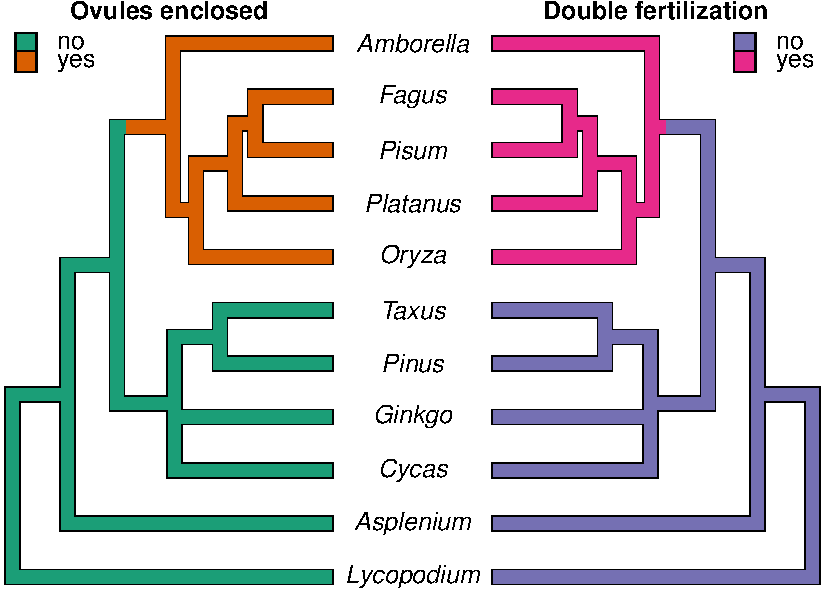
\includegraphics{pcm-workshop_files/figure-latex/AngiospermsWithCharacters4-1} \end{center}

If there are multiple species with ovules enclosed or not and that perform double fertilization or not, the most parsimonious scenario for both characters is that each evolved once along the branch of the tree that leads to the flowering plants. In other words, there has been only one transition between the states of each character in the evolution of this group.

So even if there seems to be replication when we look at the species (several species with each character state was sampled), there is no evolutionary replication! So even if the likelihood that those two events occurred on the same branch is very small and even if a contingency test to calculate the likelihood of such an event is significant, this is a little bit like an experiment with one replicate. Therefore, even when a test that accounts for the phylogeny is significant, a lot of caution is needed when interpreting these results. Ideally, a study should have a decent number of evolutionary replications for the results to be biologically meaningful. I encourage you to read the very nice paper of Maddison and Fitzjohn on the subject \citep{maddison2015unsolved}.

Ideally, before planning an experiment, one should make sure that there is sufficient replication in the evolution of the traits under study among the species considered to have greater confidence in the results. For instance, it would be much better if each character would have evolved 5-6 times each in the previous example, especially if the two characters were always evolving simultaneously!

\chapter{The Brownian Motion (BM) model}\label{BM-model}

When we want to account for the non-independence of species due to their evolutionary histories in statistical analyses, a model of evolution is necessarily implied. Indeed, we assume that traits evolved through time (along the phylogeny) and that closely related species are more likely to be more similar on average at a given trait than distantly related species. In evolutionary biologogy, the more basic model (often used as a null model in many analyses) is the Brownian motion model. This model of evolution is named after Robert Brown, a celeb botanist that published an important Flora of Australia in 1810. He was also the first to distinguish gymnosperms from angiosperms. His discovery of the Brownian motion is due to the observation that small particules in solution have the tendency to move in any direction, an observation first made while observing \emph{Clarkia} pollen under a microscope. The explanation would come later, in terms of random molecular impacts.

Mathematicians have constructed a stochastic process that is intended to approximate the Brownian motion. In this model, each step is independent from the others and can go in any direction. The mean displacement is zero and the variance is uniform across the parameter space. The displacements can be summed, which means that the variances of the independent displacements can be added up. If \(\sigma^2\) is the variance of a single displacement, the variance after time \(t\) will be \(\sigma^2t\). When the number of steps is large, as in a phylogenetic context, the result is normally distributed.

When applied to phylogenies, the Brownian motion model is kind of applied indepenpenty to each branch of the phylogeny. That allows to model the amount of change that occured along a given branch. If the variance of the Brownian motion model is \(\sigma^2\) per unit of time \(t\), then the net change along a branch of time \(t\) is drawn from a normal distribution with mean \(0\) and variance \(\sigma^2t\). This model can also be represented mathematically the following way, such as the amount of change for character \(X\) over the infinitesimal time in the interval between time \(t\) and \(t+dt\) is:

\[dX(t)=\sigma^2 dB(t),\]

where \(dB(t)\) is the gaussian distribution. Importantly, this model assumes that:

\begin{enumerate}
\def\labelenumi{\arabic{enumi}.}
\tightlist
\item
  Evolution occuring in each branch of the phylogeny is independent of that occuring in other branches.
\item
  Evolution is completely random (i.e., no selection).
\end{enumerate}

The parameter \(\sigma^2\) in the model gives the variance, or in other word the speed of evolution. The higher the variance, the faster the character will evolve. Here are two examples of simulated characters on a tree of 200 species with \(\sigma^2=0.5\) and \(\sigma^2=4\).

\begin{center}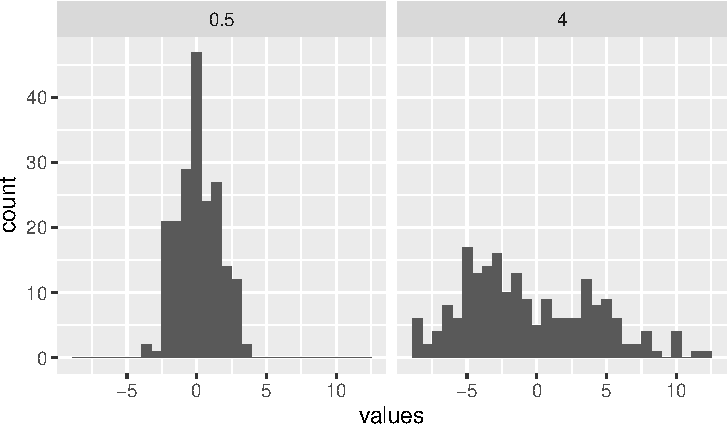
\includegraphics{pcm-workshop_files/figure-latex/BM_Model_SigmaExample-1} \end{center}

A more thorough introduction to the Brownian Motion model can be found in chapter 23 of Joe Felsenstein's book \citep{felsenstein2004inferring}.

The Brownian motion model is often said to model neutral drift, although a good fit to this model does not necessarily means that the data evolved via random drifts as other processes can also result in BM-like patterns \citep{hansen1996translating}.

Note also that the model is stochastic. That is, even if two closely related species are more likely to share similar character states than a distant one, this is only true on average. For any given simulated character, closely related species can sometimes be more different than to a distant species. Look at the following figure, that shows three traits simulated under the Brownian motion.

\begin{center}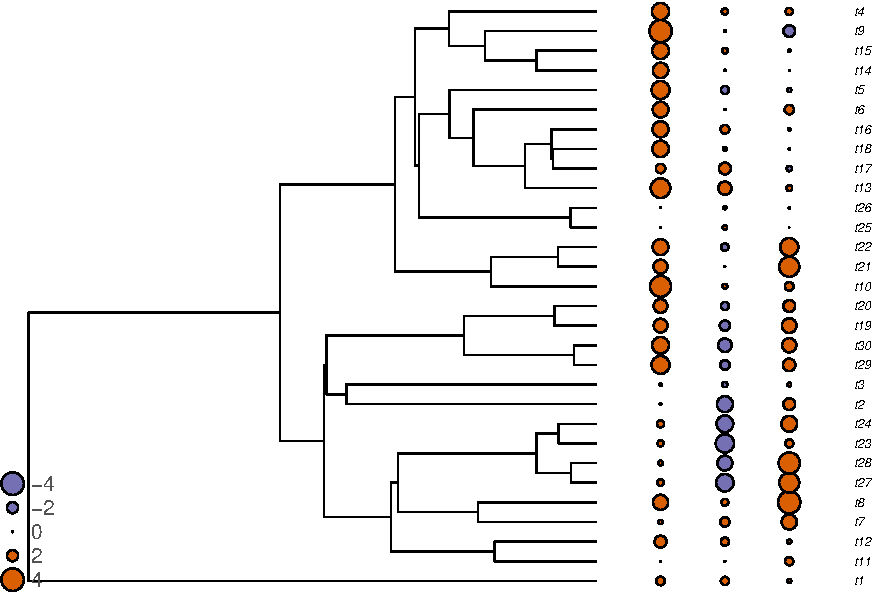
\includegraphics{pcm-workshop_files/figure-latex/PlotContinuousParameter_tablephylo4d-1} \end{center}

\chapter{Further readings}\label{further-readings}

To undertand well a new research field, it is always advisable to read a lot on it. Here are some references that you might find useful. The different sources also sometimes explain the theory in different ways or use different examples, which might help you understand better.

\begin{itemize}
\tightlist
\item
  Felsenstein, J. (1985) Phylogenies and the comparative method. \emph{The American Naturalist} 125, 1-15. \textbf{The classic initial paper that launched the field of comparative analyses. The phylogenetic independent contrasts are introduced here}
\item
  Felsenstein, J. (2004) \emph{Inferring phylogenies}. Sinauer Associates, Inc.~Sunderland, MA. \textbf{A thorough reference on phylogenies, from reconstruction to phylogenetic methods}
\item
  Hadfield, J. D., S. Nakagawa. 2010. General quantitative genetic methods for comparative biology: phylogenies, taxonomies and multi-trait models for continuous and categorical characters. \emph{Journal of Evolutionary Biology} 23:494--508. \textbf{This paper describes the phylogenetic mixed model and its implementation in MCMCglmm. It is a very important paper}
\item
  Housworth, E.A., E.P. Martins, M. Lynch. 2004. The phylogenetic mixed model. \emph{The American Naturalist} 163:84--96. \textbf{Excellent paper on the Phylogenetic Mixed Model}
\item
  Paradis, E. (2012). \emph{Analysis of phylogenetics and evolution with R}. New York, USA: Springer. \textbf{This is the book that explains the analyses available in the R package APE. It is also a great reference on many phylogenetic analyses, including the comparative method. This is a classic and a must for users of phylogenies in R.}
\item
  Revell, L J. (2010). Phylogenetic signal and linear regression on species data. \emph{Methods in Ecology and Evolution} 1: 319-329. \textbf{A great paper on PGLS. It uses simulations to show when it is important to use PGLS.}
\item
  Villemereuil, P., S. Nakagawa. 2014. General quantitative genetic methods for comparative biology. Pp. 287--303 in L. Z. Garamszegi, ed.~\emph{Modern phylogenetic comparative methods and their application in evolutionary biology}. Springer-Verlag, Berlin, Heidelberg. \textbf{Nice book chapter explaining the phylogenetic mixed model}
\item
  Zuur, A.F., E.N. Ieno, N. Walker, A. A. Saveliev, G.M. Smith. (2009). \emph{Mixed effects models and extensions in ecology with R}. New York, NY: Springer New York. \textbf{This is not a book on phylogenetic methods, but it is a great book on the analysis of ecological data with examples in R. Its chapter 6 and 7 discuss correlation structures and although they are not about phylogenies, they are very instructive on how to deal with them and how to compare models and analyse complex data. It also has tons of information on how to deal with more complex data, along with correlation structure. A very good read!}
\end{itemize}

\chapter{Introduction to phylogenies in R}\label{trees}

There are lots of packages for phylogenetic analyses in R. I won't enumerate them all here, but you can have a good idea of the options available by looking at the \href{http://cran.r-project.org/web/views/Phylogenetics.html}{phylogenetic R vignette} maintainned by Brian O'Meara. It is mostly oriented towards phylogenetic comparative methods, but it is a good start.

The most basic package for using trees in R is \emph{ape}, which allows you to read and plot trees.

\section{Importing and plotting trees}\label{importing-and-plotting-trees}

\subsection{Simulate a tree}\label{simulate-a-tree}

Throughout these exercises, we will often use simulated trees, which are very useful for pedagogical purposes. Trees can be simulated using several functions, but here is an example to simulate one tree with 15 species.

\begin{Shaded}
\begin{Highlighting}[]
\FunctionTok{require}\NormalTok{(phytools)}
\NormalTok{tree }\OtherTok{\textless{}{-}} \FunctionTok{pbtree}\NormalTok{(}\AttributeTok{n=}\DecValTok{15}\NormalTok{,}\AttributeTok{nsim=}\DecValTok{1}\NormalTok{)}
\FunctionTok{plot}\NormalTok{(tree)}
\end{Highlighting}
\end{Shaded}

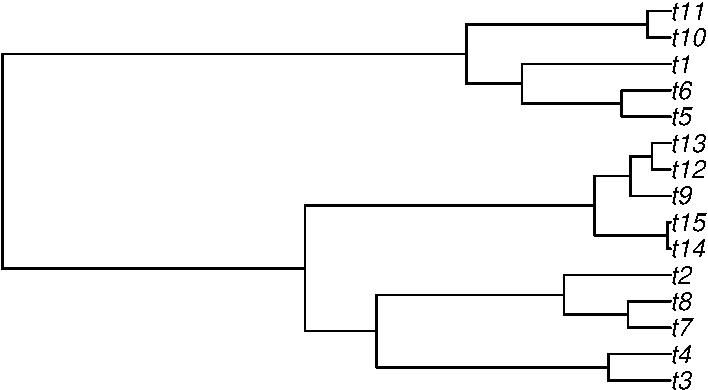
\includegraphics{pcm-workshop_files/figure-latex/Simulate Pure-Birth Tree-1.pdf}

You save the tree in nexus format to a file. But before you do so, it is a good idea to set the working directory to the same folder where your script is saved. You can do that in RStudio in the menu Session\textgreater Set Working Directory\textgreater To Source File Location.

\begin{Shaded}
\begin{Highlighting}[]
\FunctionTok{require}\NormalTok{(ape)}
\FunctionTok{write.nexus}\NormalTok{(tree, }\AttributeTok{file=}\StringTok{"My\_first\_tree.tre"}\NormalTok{)}
\end{Highlighting}
\end{Shaded}

\subsection{Simulating characters}\label{simulating-characters}

Characters can also be easily simulated in R. For instance, you could simulate a character using a Brownian Motion (BM) model using the following code.

\begin{Shaded}
\begin{Highlighting}[]
\NormalTok{trait1 }\OtherTok{\textless{}{-}} \FunctionTok{fastBM}\NormalTok{(tree, }\AttributeTok{sig2=}\FloatTok{0.01}\NormalTok{, }\AttributeTok{nsim=}\DecValTok{1}\NormalTok{, }\AttributeTok{internal=}\ConstantTok{FALSE}\NormalTok{)}
\CommentTok{\# To get trait values for tree tips:}
\NormalTok{trait1}
\end{Highlighting}
\end{Shaded}

\begin{verbatim}
##           t3           t4           t7           t8           t2          t14 
## -0.007306853  0.043251831  0.004858391 -0.114795593 -0.043737891  0.113964926 
##          t15           t9          t12          t13           t5           t6 
##  0.097243984  0.096978766  0.063069656  0.053040643  0.072476832  0.034675083 
##           t1          t10          t11 
## -0.084659118  0.118596501  0.059071786
\end{verbatim}

Now, let's save this trait to a file to pretend it is our original data.

\begin{Shaded}
\begin{Highlighting}[]
\FunctionTok{write.table}\NormalTok{(}\FunctionTok{matrix}\NormalTok{(trait1,}\AttributeTok{ncol=}\DecValTok{1}\NormalTok{,}\AttributeTok{dimnames=}\FunctionTok{list}\NormalTok{(}\FunctionTok{names}\NormalTok{(trait1),}\StringTok{"trait1"}\NormalTok{)), }\AttributeTok{file=}\StringTok{"mytrait.csv"}\NormalTok{, }\AttributeTok{sep=}\StringTok{";"}\NormalTok{)}
\end{Highlighting}
\end{Shaded}

Now that we have simulated a tree and a character, let's erase what we have done so far from the R environment and pretend these are our data for the next sections.

\begin{Shaded}
\begin{Highlighting}[]
\FunctionTok{rm}\NormalTok{(tree, trait1)}
\end{Highlighting}
\end{Shaded}

\section{Import data into R}\label{import-data-into-r}

Here is how you should import your data into R.

\begin{Shaded}
\begin{Highlighting}[]
\NormalTok{tree }\OtherTok{\textless{}{-}} \FunctionTok{read.nexus}\NormalTok{(}\AttributeTok{file=}\StringTok{"My\_first\_tree.tre"}\NormalTok{)}
\NormalTok{trait1 }\OtherTok{\textless{}{-}} \FunctionTok{read.csv2}\NormalTok{(}\AttributeTok{file=}\StringTok{"mytrait.csv"}\NormalTok{,}\AttributeTok{dec=}\StringTok{"."}\NormalTok{)}
\end{Highlighting}
\end{Shaded}

The tree format in ape contains several information and it is useful to know how to access them. For instance, the tip labels can be accessed using \texttt{tree\$tip.label} and the branch lengths using \texttt{tree\$edge.length}. Will will see more options in other exercises, but if you want more detailed information on how the objects ``phylo'' are organized, you can have a look the help file \texttt{?read.tree} or at this \href{http://ape-package.ird.fr/misc/FormatTreeR_24Oct2012.pdf}{document} prepared by Emmanuel Paradis, the author of \texttt{ape}.

\section{Plot trees}\label{plot-trees}

Plotting trees is one of the very interesting aspects of using R. Options are numerous and possibilities large. The most common function is \texttt{plot.phylo} from the ape package that has a lot of different options. I strongly suggest that you take a close look at the different options of the function \texttt{?plot.phylo}. Here is a basic example.

\begin{Shaded}
\begin{Highlighting}[]
\FunctionTok{plot}\NormalTok{(tree, }\AttributeTok{type=}\StringTok{"c"}\NormalTok{)}
\FunctionTok{add.scale.bar}\NormalTok{()}
\end{Highlighting}
\end{Shaded}

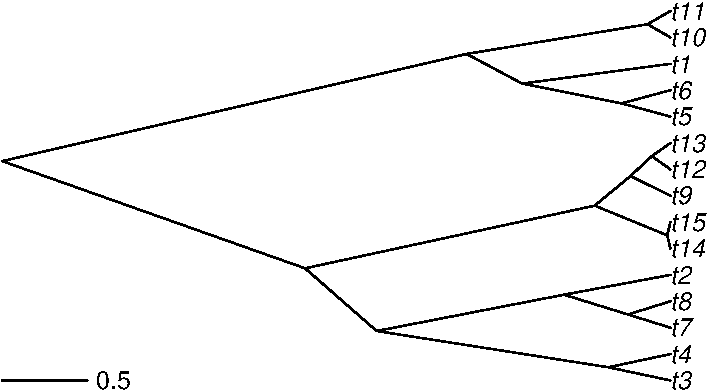
\includegraphics{pcm-workshop_files/figure-latex/Basic tree plotting-1.pdf}

But R is also interesting to plot characters alongside trees. If you have a categorical character, you could use it to color the tips of the phylogeny.

\begin{Shaded}
\begin{Highlighting}[]
\CommentTok{\# Generate a random categorical character}
\NormalTok{trait2 }\OtherTok{\textless{}{-}} \FunctionTok{as.factor}\NormalTok{(}\FunctionTok{sample}\NormalTok{(}\FunctionTok{c}\NormalTok{(}\DecValTok{1}\NormalTok{,}\DecValTok{2}\NormalTok{,}\DecValTok{3}\NormalTok{),}\AttributeTok{size=}\FunctionTok{length}\NormalTok{(tree}\SpecialCharTok{$}\NormalTok{tip.label),}\AttributeTok{replace=}\ConstantTok{TRUE}\NormalTok{))}
\CommentTok{\# Create color palette}
\FunctionTok{library}\NormalTok{(RColorBrewer)}
\NormalTok{ColorPalette1 }\OtherTok{\textless{}{-}} \FunctionTok{brewer.pal}\NormalTok{(}\AttributeTok{n =} \FunctionTok{length}\NormalTok{(}\FunctionTok{levels}\NormalTok{(trait2)), }\AttributeTok{name =} \StringTok{"Dark2"}\NormalTok{)}
\FunctionTok{plot}\NormalTok{(tree, }\AttributeTok{type=}\StringTok{"p"}\NormalTok{, }\AttributeTok{use.edge.length =} \ConstantTok{TRUE}\NormalTok{, }\AttributeTok{label.offset=}\FloatTok{0.2}\NormalTok{,}\AttributeTok{cex=}\DecValTok{1}\NormalTok{)}
\FunctionTok{tiplabels}\NormalTok{(}\AttributeTok{pch=}\DecValTok{21}\NormalTok{,}\AttributeTok{bg=}\NormalTok{ColorPalette1[trait2],}\AttributeTok{col=}\StringTok{"black"}\NormalTok{,}\AttributeTok{cex=}\DecValTok{1}\NormalTok{,}\AttributeTok{adj=}\FloatTok{0.6}\NormalTok{)}
\NormalTok{op}\OtherTok{\textless{}{-}}\FunctionTok{par}\NormalTok{(}\AttributeTok{xpd=}\ConstantTok{TRUE}\NormalTok{)}
\FunctionTok{legend}\NormalTok{(}\DecValTok{0}\NormalTok{,}\DecValTok{0}\NormalTok{,}\AttributeTok{legend=}\FunctionTok{levels}\NormalTok{(trait2),}\AttributeTok{col=}\NormalTok{ColorPalette1,}
       \AttributeTok{pch=}\DecValTok{20}\NormalTok{,}\AttributeTok{bty=}\StringTok{"n"}\NormalTok{,}\AttributeTok{cex=}\DecValTok{1}\NormalTok{,}\AttributeTok{pt.cex=}\FloatTok{1.5}\NormalTok{,}\AttributeTok{ncol=}\FunctionTok{length}\NormalTok{(}\FunctionTok{levels}\NormalTok{(trait2)))}
\end{Highlighting}
\end{Shaded}

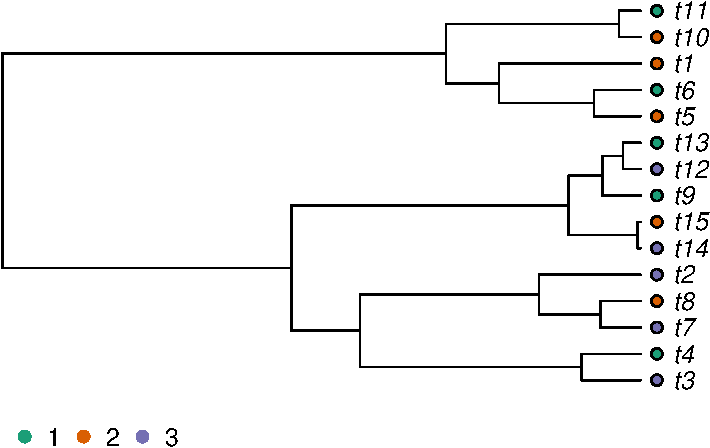
\includegraphics{pcm-workshop_files/figure-latex/Plot categorical parameter-1.pdf}

\begin{Shaded}
\begin{Highlighting}[]
\FunctionTok{par}\NormalTok{(op) }\CommentTok{\#reset graphical parameters to defaults}
\end{Highlighting}
\end{Shaded}

A similar result could be obtained with a continuous variable. Here, we will use the Brownian Motion model, which we will study in a further class, to simulate the continuous character.

\begin{Shaded}
\begin{Highlighting}[]
\CommentTok{\# Breakdown continuous trait in categories}
\NormalTok{trait1.cat }\OtherTok{\textless{}{-}} \FunctionTok{cut}\NormalTok{(trait1[,}\DecValTok{1}\NormalTok{],}\AttributeTok{breaks=}\DecValTok{8}\NormalTok{,}\AttributeTok{labels=}\ConstantTok{FALSE}\NormalTok{)}
\CommentTok{\# Create color palette}
\NormalTok{ColorPalette2 }\OtherTok{\textless{}{-}} \FunctionTok{brewer.pal}\NormalTok{(}\AttributeTok{n =} \DecValTok{8}\NormalTok{, }\AttributeTok{name =} \StringTok{"Blues"}\NormalTok{)}
\CommentTok{\# Plot the tree}
\FunctionTok{plot}\NormalTok{(tree, }\AttributeTok{type=}\StringTok{"p"}\NormalTok{, }\AttributeTok{use.edge.length =} \ConstantTok{TRUE}\NormalTok{, }\AttributeTok{label.offset=}\FloatTok{0.2}\NormalTok{,}\AttributeTok{cex=}\DecValTok{1}\NormalTok{)}
\FunctionTok{tiplabels}\NormalTok{(}\AttributeTok{pch=}\DecValTok{21}\NormalTok{,}\AttributeTok{bg=}\NormalTok{ColorPalette2[trait1.cat],}\AttributeTok{col=}\StringTok{"black"}\NormalTok{,}\AttributeTok{cex=}\DecValTok{1}\NormalTok{,}\AttributeTok{adj=}\FloatTok{0.6}\NormalTok{)}
\NormalTok{op}\OtherTok{\textless{}{-}}\FunctionTok{par}\NormalTok{(}\AttributeTok{xpd=}\ConstantTok{TRUE}\NormalTok{)}
\FunctionTok{legend}\NormalTok{(}\DecValTok{0}\NormalTok{,}\DecValTok{0}\NormalTok{,}\AttributeTok{legend=}\FunctionTok{levels}\NormalTok{(}\FunctionTok{cut}\NormalTok{(trait1[,}\DecValTok{1}\NormalTok{],}\AttributeTok{breaks=}\DecValTok{8}\NormalTok{)),}
       \AttributeTok{col=}\NormalTok{ColorPalette2,}\AttributeTok{pch=}\DecValTok{20}\NormalTok{,}\AttributeTok{bty=}\StringTok{"n"}\NormalTok{,}\AttributeTok{cex=}\FloatTok{0.7}\NormalTok{,}\AttributeTok{pt.cex=}\FloatTok{1.5}\NormalTok{,}\AttributeTok{ncol=}\DecValTok{4}\NormalTok{)}
\end{Highlighting}
\end{Shaded}

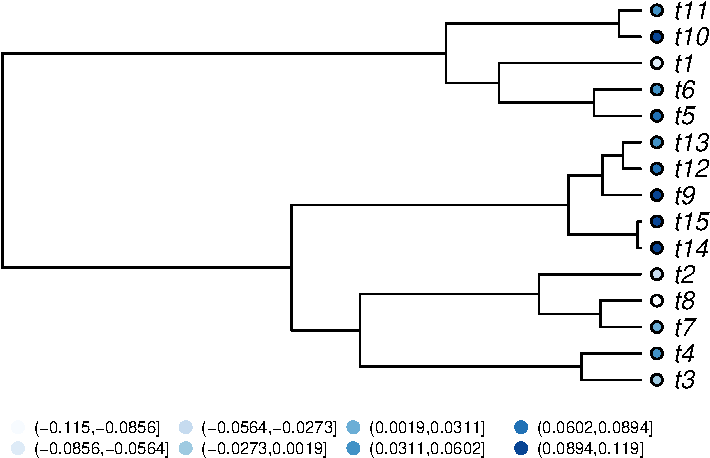
\includegraphics{pcm-workshop_files/figure-latex/Plot continuous parameter-1.pdf}

\begin{Shaded}
\begin{Highlighting}[]
\FunctionTok{par}\NormalTok{(op) }\CommentTok{\#reset graphical parameters to defaults}
\end{Highlighting}
\end{Shaded}

As expected from a character simlated with Brownian motion, you can see that closely related species tend to have more similar character values.

Another option to represent a continuous parameter is to use the function \texttt{table.phylo4d} from the \texttt{adephylo} package to represent the trait where its values are represented by sizes of different sizes and colors. It is also possible to plot multiple characters at the same time.

Note that you will have to install the packages \texttt{phylobase} and \texttt{adephylo} to run these function if they are not installed.

\begin{Shaded}
\begin{Highlighting}[]
\FunctionTok{library}\NormalTok{(phylobase)}
\FunctionTok{library}\NormalTok{(adephylo)}
\NormalTok{trait3 }\OtherTok{\textless{}{-}} \FunctionTok{fastBM}\NormalTok{(tree, }\AttributeTok{sig2=}\FloatTok{0.1}\NormalTok{, }\AttributeTok{nsim=}\DecValTok{1}\NormalTok{, }\AttributeTok{internal=}\ConstantTok{FALSE}\NormalTok{) }\CommentTok{\#simulate a faster evolving trait}
\NormalTok{trait.table }\OtherTok{\textless{}{-}} \FunctionTok{data.frame}\NormalTok{(}\AttributeTok{trait1=}\NormalTok{trait1[,}\DecValTok{1}\NormalTok{], trait3)}
\NormalTok{obj }\OtherTok{\textless{}{-}} \FunctionTok{phylo4d}\NormalTok{(tree, trait.table) }\CommentTok{\# build a phylo4d object}
\NormalTok{op }\OtherTok{\textless{}{-}} \FunctionTok{par}\NormalTok{(}\AttributeTok{mar=}\FunctionTok{c}\NormalTok{(}\DecValTok{1}\NormalTok{,}\DecValTok{1}\NormalTok{,}\DecValTok{1}\NormalTok{,}\DecValTok{1}\NormalTok{))}
\FunctionTok{table.phylo4d}\NormalTok{(obj,}\AttributeTok{cex.label=}\DecValTok{1}\NormalTok{,}\AttributeTok{cex.symbol=}\DecValTok{1}\NormalTok{,}\AttributeTok{ratio.tree=}\FloatTok{0.8}\NormalTok{,}\AttributeTok{grid=}\ConstantTok{FALSE}\NormalTok{,}\AttributeTok{box=}\ConstantTok{FALSE}\NormalTok{)}
\end{Highlighting}
\end{Shaded}

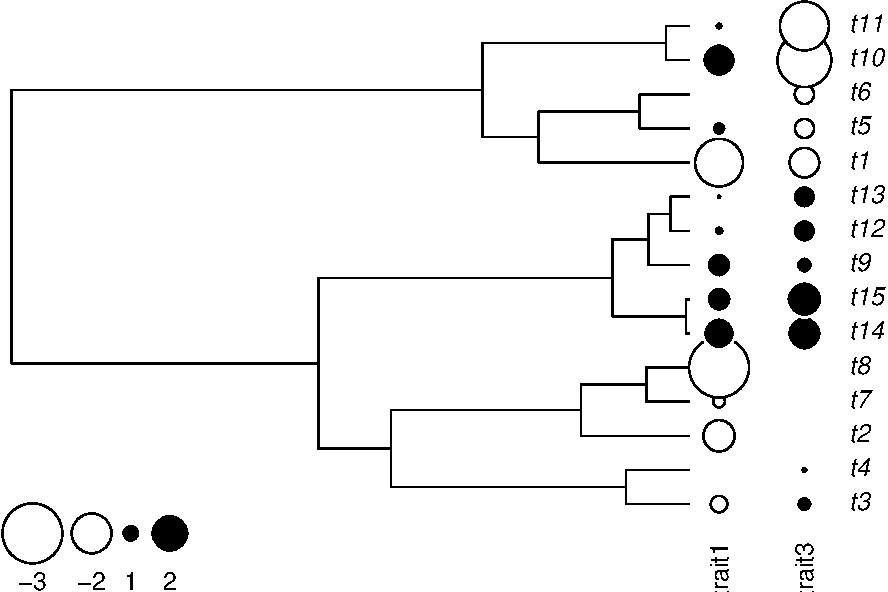
\includegraphics{pcm-workshop_files/figure-latex/Plot continuous parameter - table.phylo4d-1.pdf}

\begin{Shaded}
\begin{Highlighting}[]
\FunctionTok{par}\NormalTok{(op) }\CommentTok{\#reset graphical parameters to defaults}
\end{Highlighting}
\end{Shaded}

You can also represent a traitgram:

\begin{Shaded}
\begin{Highlighting}[]
\FunctionTok{require}\NormalTok{(phytools)}
\FunctionTok{phenogram}\NormalTok{(tree,trait3,}\AttributeTok{spread.labels=}\ConstantTok{TRUE}\NormalTok{)}
\end{Highlighting}
\end{Shaded}

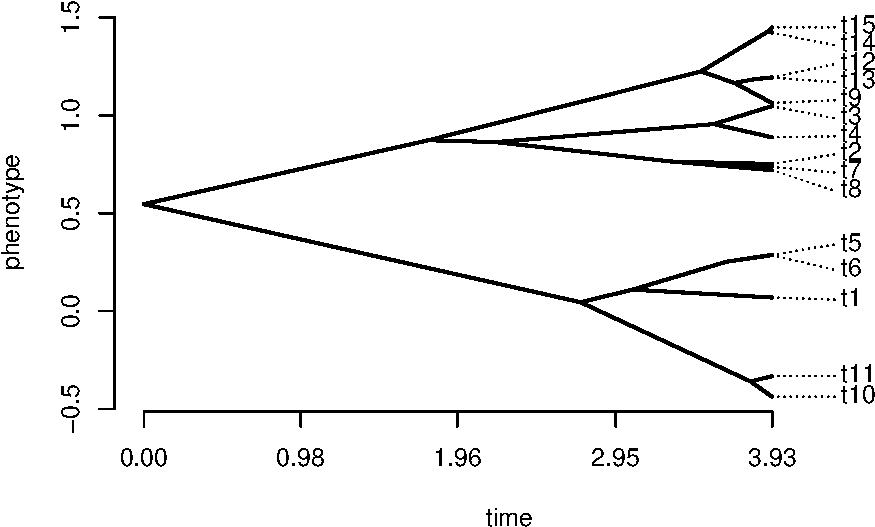
\includegraphics{pcm-workshop_files/figure-latex/traitgram-1.pdf}

Finally, it is also possible to represent a tree on a 2-dimensional plot, coloring points with the categorical variable.

\begin{Shaded}
\begin{Highlighting}[]
\FunctionTok{phylomorphospace}\NormalTok{(tree,trait.table)}
\FunctionTok{points}\NormalTok{(trait.table,}\AttributeTok{pch=}\DecValTok{21}\NormalTok{,}\AttributeTok{bg=}\NormalTok{ColorPalette1[trait2],}\AttributeTok{col=}\StringTok{"black"}\NormalTok{,}\AttributeTok{cex=}\FloatTok{1.2}\NormalTok{,}\AttributeTok{adj=}\DecValTok{1}\NormalTok{)}
\FunctionTok{legend}\NormalTok{(}\StringTok{"topleft"}\NormalTok{,}\AttributeTok{legend=}\FunctionTok{levels}\NormalTok{(trait2),}
       \AttributeTok{col=}\NormalTok{ColorPalette1,}\AttributeTok{pch=}\DecValTok{20}\NormalTok{,}\AttributeTok{bty=}\StringTok{"n"}\NormalTok{,}\AttributeTok{cex=}\DecValTok{1}\NormalTok{,}\AttributeTok{pt.cex=}\FloatTok{1.5}\NormalTok{,}\AttributeTok{ncol=}\FunctionTok{length}\NormalTok{(}\FunctionTok{levels}\NormalTok{(trait2)))}
\end{Highlighting}
\end{Shaded}

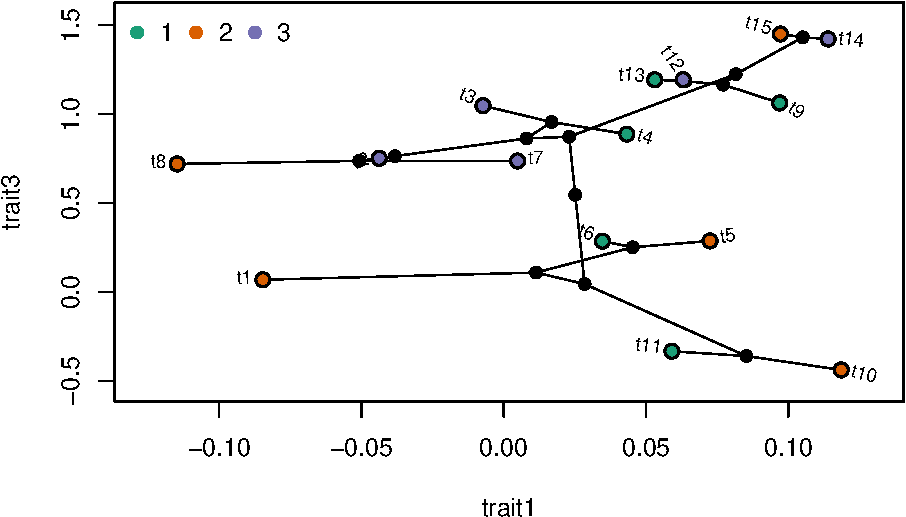
\includegraphics{pcm-workshop_files/figure-latex/Phylomorphospace-1.pdf}

\section{Handling multiple trees}\label{handling-multiple-trees}

In several cases, it is important to know how to handle multiple trees in R. These are normally stored in a \texttt{multiPhylo} object. Let's see an example.

\begin{Shaded}
\begin{Highlighting}[]
\NormalTok{trees }\OtherTok{\textless{}{-}} \FunctionTok{pbtree}\NormalTok{(}\AttributeTok{n=}\DecValTok{15}\NormalTok{,}\AttributeTok{nsim=}\DecValTok{10}\NormalTok{)}
\NormalTok{trees}
\end{Highlighting}
\end{Shaded}

\begin{verbatim}
## 10 phylogenetic trees
\end{verbatim}

You can see that the object is not the same as a phylo object. For instance, if you use the code \texttt{plot(trees)}, you will be prompted to hit enter to pass from one tree to the other. To access to individual trees, you need to use the following technique.

\begin{Shaded}
\begin{Highlighting}[]
\NormalTok{trees[[}\DecValTok{1}\NormalTok{]]}
\end{Highlighting}
\end{Shaded}

\begin{verbatim}
## 
## Phylogenetic tree with 15 tips and 14 internal nodes.
## 
## Tip labels:
##   t3, t4, t5, t14, t15, t8, ...
## 
## Rooted; includes branch lengths.
\end{verbatim}

\begin{Shaded}
\begin{Highlighting}[]
\FunctionTok{plot}\NormalTok{(trees[[}\DecValTok{1}\NormalTok{]])}
\end{Highlighting}
\end{Shaded}

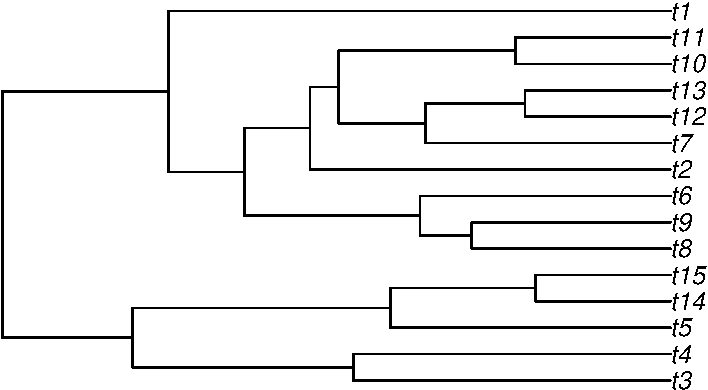
\includegraphics{pcm-workshop_files/figure-latex/multiPhylo manipulation-1.pdf}

\section{Manipulating trees}\label{manipulating-trees}

There are several manipulations that can be made to trees. Here are a few examples.

\subsection{Drop tips}\label{drop-tips}

\begin{Shaded}
\begin{Highlighting}[]
\FunctionTok{plot}\NormalTok{(}\FunctionTok{drop.tip}\NormalTok{(tree,}\FunctionTok{c}\NormalTok{(}\StringTok{"t1"}\NormalTok{,}\StringTok{"t2"}\NormalTok{,}\StringTok{"t3"}\NormalTok{,}\StringTok{"t4"}\NormalTok{,}\StringTok{"t5"}\NormalTok{)))}
\end{Highlighting}
\end{Shaded}

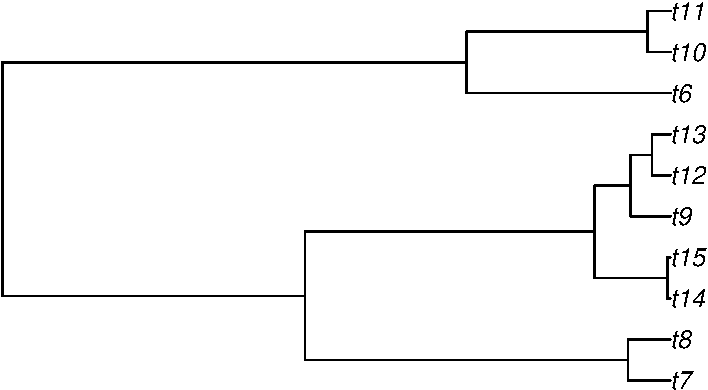
\includegraphics{pcm-workshop_files/figure-latex/Drop tips-1.pdf}

\subsection{Reroot trees}\label{reroot-trees}

\begin{Shaded}
\begin{Highlighting}[]
\FunctionTok{plot}\NormalTok{(}\FunctionTok{root}\NormalTok{(tree,}\StringTok{"t1"}\NormalTok{))}
\end{Highlighting}
\end{Shaded}

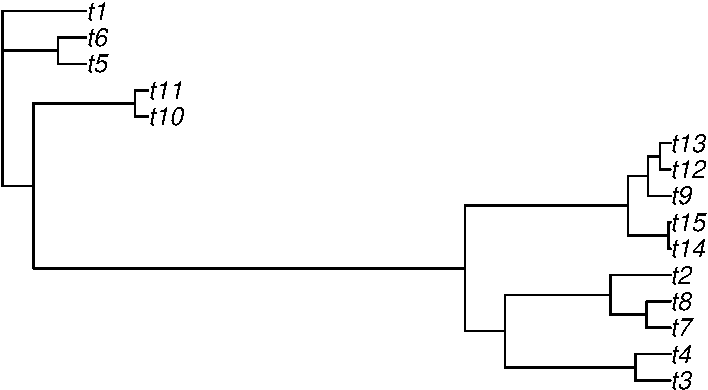
\includegraphics{pcm-workshop_files/figure-latex/Reroot trees-1.pdf}

\subsection{Get cophenetic distances}\label{get-cophenetic-distances}

\begin{Shaded}
\begin{Highlighting}[]
\FunctionTok{cophenetic.phylo}\NormalTok{(tree)}
\end{Highlighting}
\end{Shaded}

\begin{verbatim}
##            t3        t4        t7        t8       t2        t14        t15
## t3  0.0000000 0.7285289 3.4533793 3.4533793 3.453379 4.29496600 4.29496600
## t4  0.7285289 0.0000000 3.4533793 3.4533793 3.453379 4.29496600 4.29496600
## t7  3.4533793 3.4533793 0.0000000 0.4962115 1.250834 4.29496600 4.29496600
## t8  3.4533793 3.4533793 0.4962115 0.0000000 1.250834 4.29496600 4.29496600
## t2  3.4533793 3.4533793 1.2508336 1.2508336 0.000000 4.29496600 4.29496600
## t14 4.2949660 4.2949660 4.2949660 4.2949660 4.294966 0.00000000 0.03691962
## t15 4.2949660 4.2949660 4.2949660 4.2949660 4.294966 0.03691962 0.00000000
## t9  4.2949660 4.2949660 4.2949660 4.2949660 4.294966 0.88909442 0.88909442
## t12 4.2949660 4.2949660 4.2949660 4.2949660 4.294966 0.88909442 0.88909442
## t13 4.2949660 4.2949660 4.2949660 4.2949660 4.294966 0.88909442 0.88909442
## t5  7.8556290 7.8556290 7.8556290 7.8556290 7.855629 7.85562897 7.85562897
## t6  7.8556290 7.8556290 7.8556290 7.8556290 7.855629 7.85562897 7.85562897
## t1  7.8556290 7.8556290 7.8556290 7.8556290 7.855629 7.85562897 7.85562897
## t10 7.8556290 7.8556290 7.8556290 7.8556290 7.855629 7.85562897 7.85562897
## t11 7.8556290 7.8556290 7.8556290 7.8556290 7.855629 7.85562897 7.85562897
##            t9       t12       t13        t5        t6       t1      t10
## t3  4.2949660 4.2949660 4.2949660 7.8556290 7.8556290 7.855629 7.855629
## t4  4.2949660 4.2949660 4.2949660 7.8556290 7.8556290 7.855629 7.855629
## t7  4.2949660 4.2949660 4.2949660 7.8556290 7.8556290 7.855629 7.855629
## t8  4.2949660 4.2949660 4.2949660 7.8556290 7.8556290 7.855629 7.855629
## t2  4.2949660 4.2949660 4.2949660 7.8556290 7.8556290 7.855629 7.855629
## t14 0.8890944 0.8890944 0.8890944 7.8556290 7.8556290 7.855629 7.855629
## t15 0.8890944 0.8890944 0.8890944 7.8556290 7.8556290 7.855629 7.855629
## t9  0.0000000 0.4685481 0.4685481 7.8556290 7.8556290 7.855629 7.855629
## t12 0.4685481 0.0000000 0.2174902 7.8556290 7.8556290 7.855629 7.855629
## t13 0.4685481 0.2174902 0.0000000 7.8556290 7.8556290 7.855629 7.855629
## t5  7.8556290 7.8556290 7.8556290 0.0000000 0.5720997 1.742611 2.395633
## t6  7.8556290 7.8556290 7.8556290 0.5720997 0.0000000 1.742611 2.395633
## t1  7.8556290 7.8556290 7.8556290 1.7426110 1.7426110 0.000000 2.395633
## t10 7.8556290 7.8556290 7.8556290 2.3956328 2.3956328 2.395633 0.000000
## t11 7.8556290 7.8556290 7.8556290 2.3956328 2.3956328 2.395633 0.268201
##          t11
## t3  7.855629
## t4  7.855629
## t7  7.855629
## t8  7.855629
## t2  7.855629
## t14 7.855629
## t15 7.855629
## t9  7.855629
## t12 7.855629
## t13 7.855629
## t5  2.395633
## t6  2.395633
## t1  2.395633
## t10 0.268201
## t11 0.000000
\end{verbatim}

\chapter{Solutions to the challenges}\label{solutions}

\section{Challenge 1}\label{challenge-1-1}

In the \texttt{seedplantsdata} data frame, there were many different traits. Try to fit a regression of tree shade tolerance (\texttt{shade}) on the seed mass (\texttt{Sm}). In other words, test if shade tolerance can be explained by the seed mass of the trees. Then, try to see if the residuals are phylogenetically correlated.

\begin{Shaded}
\begin{Highlighting}[]
\CommentTok{\# Fit a linear model using Ordinary Least Squares (OLS)}
\NormalTok{Sm.lm }\OtherTok{\textless{}{-}} \FunctionTok{lm}\NormalTok{(Shade }\SpecialCharTok{\textasciitilde{}}\NormalTok{ Sm, }\AttributeTok{data =}\NormalTok{ seedplantsdata)}
\CommentTok{\# Get the results}
\FunctionTok{summary}\NormalTok{(Sm.lm)}
\end{Highlighting}
\end{Shaded}

\begin{verbatim}
## 
## Call:
## lm(formula = Shade ~ Sm, data = seedplantsdata)
## 
## Residuals:
##     Min      1Q  Median      3Q     Max 
## -1.9042 -0.9009  0.1481  0.5982  2.0962 
## 
## Coefficients:
##               Estimate Std. Error t value Pr(>|t|)    
## (Intercept)  2.904e+00  1.608e-01  18.064   <2e-16 ***
## Sm          -5.824e-05  5.640e-05  -1.033    0.306    
## ---
## Signif. codes:  0 '***' 0.001 '**' 0.01 '*' 0.05 '.' 0.1 ' ' 1
## 
## Residual standard error: 1.149 on 55 degrees of freedom
## Multiple R-squared:  0.01902,    Adjusted R-squared:  0.001184 
## F-statistic: 1.066 on 1 and 55 DF,  p-value: 0.3063
\end{verbatim}

\begin{Shaded}
\begin{Highlighting}[]
\CommentTok{\# Extract the residuals}
\NormalTok{Sm.res }\OtherTok{\textless{}{-}} \FunctionTok{residuals}\NormalTok{(Sm.lm)}
\CommentTok{\# Plot the residuals beside the phylogeny}
\NormalTok{op }\OtherTok{\textless{}{-}} \FunctionTok{par}\NormalTok{(}\AttributeTok{mar=}\FunctionTok{c}\NormalTok{(}\DecValTok{1}\NormalTok{,}\DecValTok{1}\NormalTok{,}\DecValTok{1}\NormalTok{,}\DecValTok{1}\NormalTok{))}
\FunctionTok{plot}\NormalTok{(seedplantstree,}\AttributeTok{type=}\StringTok{"p"}\NormalTok{,}\ConstantTok{TRUE}\NormalTok{,}\AttributeTok{label.offset=}\FloatTok{0.01}\NormalTok{,}\AttributeTok{cex=}\FloatTok{0.5}\NormalTok{,}\AttributeTok{no.margin=}\ConstantTok{FALSE}\NormalTok{)}
\FunctionTok{tiplabels}\NormalTok{(}\AttributeTok{pch=}\DecValTok{21}\NormalTok{,}\AttributeTok{bg=}\NormalTok{cols[}\FunctionTok{ifelse}\NormalTok{(Sm.res}\SpecialCharTok{\textgreater{}}\DecValTok{0}\NormalTok{,}\DecValTok{1}\NormalTok{,}\DecValTok{2}\NormalTok{)],}\AttributeTok{col=}\StringTok{"black"}\NormalTok{,}\AttributeTok{cex=}\FunctionTok{abs}\NormalTok{(Sm.res),}\AttributeTok{adj=}\FloatTok{0.505}\NormalTok{)}
\FunctionTok{legend}\NormalTok{(}\StringTok{"topleft"}\NormalTok{,}\AttributeTok{legend=}\FunctionTok{c}\NormalTok{(}\StringTok{"{-}2"}\NormalTok{,}\StringTok{"{-}1"}\NormalTok{,}\StringTok{"0"}\NormalTok{,}\StringTok{"1"}\NormalTok{,}\StringTok{"2"}\NormalTok{),}\AttributeTok{pch=}\DecValTok{21}\NormalTok{,}
       \AttributeTok{pt.bg=}\NormalTok{cols[}\FunctionTok{c}\NormalTok{(}\DecValTok{1}\NormalTok{,}\DecValTok{1}\NormalTok{,}\DecValTok{1}\NormalTok{,}\DecValTok{2}\NormalTok{,}\DecValTok{2}\NormalTok{)],}\AttributeTok{bty=}\StringTok{"n"}\NormalTok{,}
       \AttributeTok{text.col=}\StringTok{"gray32"}\NormalTok{,}\AttributeTok{cex=}\FloatTok{0.8}\NormalTok{,}\AttributeTok{pt.cex=}\FunctionTok{c}\NormalTok{(}\DecValTok{2}\NormalTok{,}\DecValTok{1}\NormalTok{,}\FloatTok{0.1}\NormalTok{,}\DecValTok{1}\NormalTok{,}\DecValTok{2}\NormalTok{))}
\end{Highlighting}
\end{Shaded}

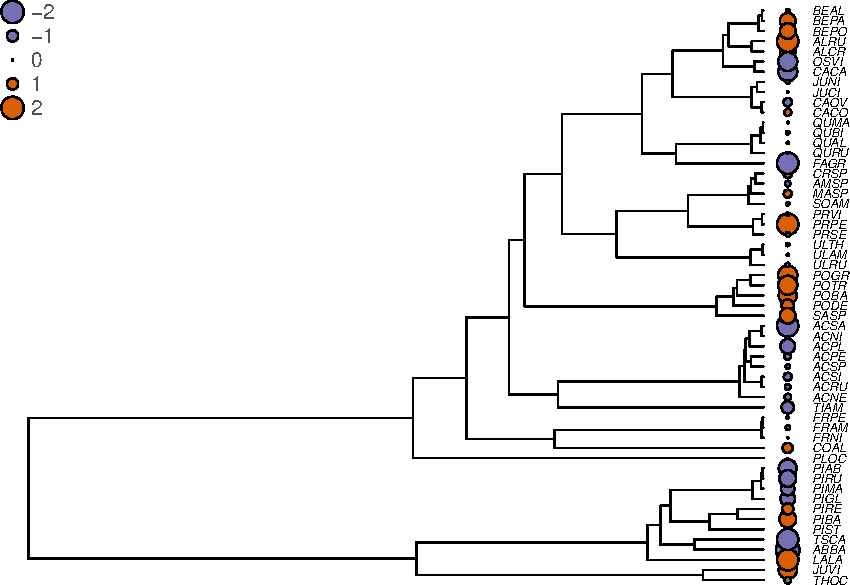
\includegraphics{pcm-workshop_files/figure-latex/Challenge 1 - solution-1.pdf}

\begin{Shaded}
\begin{Highlighting}[]
\FunctionTok{par}\NormalTok{(op)}
\end{Highlighting}
\end{Shaded}

\section{Challenge 2}\label{challenge-2-1}

Can you get the covariance matrix and the correlation matrix for the seed plants phylogenetic tree from the example above (\texttt{seedplantstree})?

\begin{Shaded}
\begin{Highlighting}[]
\CommentTok{\# Covariance matrix}
\NormalTok{seedplants.cov }\OtherTok{\textless{}{-}} \FunctionTok{vcv}\NormalTok{(seedplantstree,}\AttributeTok{corr=}\ConstantTok{FALSE}\NormalTok{)}
\CommentTok{\# Check the first few lines of the matrix}
\FunctionTok{head}\NormalTok{(}\FunctionTok{round}\NormalTok{(seedplants.cov,}\DecValTok{3}\NormalTok{))}
\end{Highlighting}
\end{Shaded}

\begin{verbatim}
##       ABBA  ACNE  ACNI  ACPE  ACPL  ACRU  ACSA  ACSI  ACSP  ALCR  ALRU  AMSP
## ABBA 0.151 0.000 0.000 0.000 0.000 0.000 0.000 0.000 0.000 0.000 0.000 0.000
## ACNE 0.000 0.151 0.146 0.146 0.146 0.146 0.146 0.146 0.146 0.099 0.099 0.099
## ACNI 0.000 0.146 0.151 0.147 0.148 0.147 0.150 0.147 0.147 0.099 0.099 0.099
## ACPE 0.000 0.146 0.147 0.151 0.147 0.147 0.147 0.147 0.148 0.099 0.099 0.099
## ACPL 0.000 0.146 0.148 0.147 0.151 0.147 0.148 0.147 0.147 0.099 0.099 0.099
## ACRU 0.000 0.146 0.147 0.147 0.147 0.151 0.147 0.150 0.147 0.099 0.099 0.099
##       BEAL  BEPA  BEPO  CACA  CACO  CAOV COAL  CRSP  FAGR FRAM FRNI FRPE  JUCI
## ABBA 0.000 0.000 0.000 0.000 0.000 0.000 0.00 0.000 0.000 0.00 0.00 0.00 0.000
## ACNE 0.099 0.099 0.099 0.099 0.099 0.099 0.09 0.099 0.099 0.09 0.09 0.09 0.099
## ACNI 0.099 0.099 0.099 0.099 0.099 0.099 0.09 0.099 0.099 0.09 0.09 0.09 0.099
## ACPE 0.099 0.099 0.099 0.099 0.099 0.099 0.09 0.099 0.099 0.09 0.09 0.09 0.099
## ACPL 0.099 0.099 0.099 0.099 0.099 0.099 0.09 0.099 0.099 0.09 0.09 0.09 0.099
## ACRU 0.099 0.099 0.099 0.099 0.099 0.099 0.09 0.099 0.099 0.09 0.09 0.09 0.099
##       JUNI JUVI  LALA  MASP  OSVI PIAB PIBA PIGL PIMA PIRE PIRU PIST  PLOC
## ABBA 0.000 0.08 0.127 0.000 0.000 0.13 0.13 0.13 0.13 0.13 0.13 0.13 0.000
## ACNE 0.099 0.00 0.000 0.099 0.099 0.00 0.00 0.00 0.00 0.00 0.00 0.00 0.079
## ACNI 0.099 0.00 0.000 0.099 0.099 0.00 0.00 0.00 0.00 0.00 0.00 0.00 0.079
## ACPE 0.099 0.00 0.000 0.099 0.099 0.00 0.00 0.00 0.00 0.00 0.00 0.00 0.079
## ACPL 0.099 0.00 0.000 0.099 0.099 0.00 0.00 0.00 0.00 0.00 0.00 0.00 0.079
## ACRU 0.099 0.00 0.000 0.099 0.099 0.00 0.00 0.00 0.00 0.00 0.00 0.00 0.079
##       POBA  PODE  POGR  POTR  PRPE  PRSE  PRVI  QUAL  QUBI  QUMA  QURU  SASP
## ABBA 0.000 0.000 0.000 0.000 0.000 0.000 0.000 0.000 0.000 0.000 0.000 0.000
## ACNE 0.099 0.099 0.099 0.099 0.099 0.099 0.099 0.099 0.099 0.099 0.099 0.099
## ACNI 0.099 0.099 0.099 0.099 0.099 0.099 0.099 0.099 0.099 0.099 0.099 0.099
## ACPE 0.099 0.099 0.099 0.099 0.099 0.099 0.099 0.099 0.099 0.099 0.099 0.099
## ACPL 0.099 0.099 0.099 0.099 0.099 0.099 0.099 0.099 0.099 0.099 0.099 0.099
## ACRU 0.099 0.099 0.099 0.099 0.099 0.099 0.099 0.099 0.099 0.099 0.099 0.099
##       SOAM THOC  TIAM  TSCA  ULAM  ULRU  ULTH
## ABBA 0.000 0.08 0.000 0.137 0.000 0.000 0.000
## ACNE 0.099 0.00 0.109 0.000 0.099 0.099 0.099
## ACNI 0.099 0.00 0.109 0.000 0.099 0.099 0.099
## ACPE 0.099 0.00 0.109 0.000 0.099 0.099 0.099
## ACPL 0.099 0.00 0.109 0.000 0.099 0.099 0.099
## ACRU 0.099 0.00 0.109 0.000 0.099 0.099 0.099
\end{verbatim}

\begin{Shaded}
\begin{Highlighting}[]
\CommentTok{\# Correlation matrix}
\NormalTok{seedplants.cor }\OtherTok{\textless{}{-}} \FunctionTok{vcv}\NormalTok{(seedplantstree,}\AttributeTok{corr=}\ConstantTok{TRUE}\NormalTok{)}
\CommentTok{\# Check the first few lines of the matrix}
\FunctionTok{head}\NormalTok{(}\FunctionTok{round}\NormalTok{(seedplants.cor,}\DecValTok{3}\NormalTok{))}
\end{Highlighting}
\end{Shaded}

\begin{verbatim}
##      ABBA  ACNE  ACNI  ACPE  ACPL  ACRU  ACSA  ACSI  ACSP  ALCR  ALRU  AMSP
## ABBA    1 0.000 0.000 0.000 0.000 0.000 0.000 0.000 0.000 0.000 0.000 0.000
## ACNE    0 1.000 0.967 0.967 0.967 0.967 0.967 0.967 0.967 0.654 0.654 0.654
## ACNI    0 0.967 1.000 0.976 0.981 0.974 0.997 0.974 0.976 0.654 0.654 0.654
## ACPE    0 0.967 0.976 1.000 0.976 0.974 0.976 0.974 0.983 0.654 0.654 0.654
## ACPL    0 0.967 0.981 0.976 1.000 0.974 0.981 0.974 0.976 0.654 0.654 0.654
## ACRU    0 0.967 0.974 0.974 0.974 1.000 0.974 0.997 0.974 0.654 0.654 0.654
##       BEAL  BEPA  BEPO  CACA  CACO  CAOV  COAL  CRSP  FAGR  FRAM  FRNI  FRPE
## ABBA 0.000 0.000 0.000 0.000 0.000 0.000 0.000 0.000 0.000 0.000 0.000 0.000
## ACNE 0.654 0.654 0.654 0.654 0.654 0.654 0.596 0.654 0.654 0.596 0.596 0.596
## ACNI 0.654 0.654 0.654 0.654 0.654 0.654 0.596 0.654 0.654 0.596 0.596 0.596
## ACPE 0.654 0.654 0.654 0.654 0.654 0.654 0.596 0.654 0.654 0.596 0.596 0.596
## ACPL 0.654 0.654 0.654 0.654 0.654 0.654 0.596 0.654 0.654 0.596 0.596 0.596
## ACRU 0.654 0.654 0.654 0.654 0.654 0.654 0.596 0.654 0.654 0.596 0.596 0.596
##       JUCI  JUNI  JUVI  LALA  MASP  OSVI PIAB PIBA PIGL PIMA PIRE PIRU PIST
## ABBA 0.000 0.000 0.528 0.843 0.000 0.000 0.86 0.86 0.86 0.86 0.86 0.86 0.86
## ACNE 0.654 0.654 0.000 0.000 0.654 0.654 0.00 0.00 0.00 0.00 0.00 0.00 0.00
## ACNI 0.654 0.654 0.000 0.000 0.654 0.654 0.00 0.00 0.00 0.00 0.00 0.00 0.00
## ACPE 0.654 0.654 0.000 0.000 0.654 0.654 0.00 0.00 0.00 0.00 0.00 0.00 0.00
## ACPL 0.654 0.654 0.000 0.000 0.654 0.654 0.00 0.00 0.00 0.00 0.00 0.00 0.00
## ACRU 0.654 0.654 0.000 0.000 0.654 0.654 0.00 0.00 0.00 0.00 0.00 0.00 0.00
##       PLOC  POBA  PODE  POGR  POTR  PRPE  PRSE  PRVI  QUAL  QUBI  QUMA  QURU
## ABBA 0.000 0.000 0.000 0.000 0.000 0.000 0.000 0.000 0.000 0.000 0.000 0.000
## ACNE 0.523 0.654 0.654 0.654 0.654 0.654 0.654 0.654 0.654 0.654 0.654 0.654
## ACNI 0.523 0.654 0.654 0.654 0.654 0.654 0.654 0.654 0.654 0.654 0.654 0.654
## ACPE 0.523 0.654 0.654 0.654 0.654 0.654 0.654 0.654 0.654 0.654 0.654 0.654
## ACPL 0.523 0.654 0.654 0.654 0.654 0.654 0.654 0.654 0.654 0.654 0.654 0.654
## ACRU 0.523 0.654 0.654 0.654 0.654 0.654 0.654 0.654 0.654 0.654 0.654 0.654
##       SASP  SOAM  THOC TIAM  TSCA  ULAM  ULRU  ULTH
## ABBA 0.000 0.000 0.528 0.00 0.906 0.000 0.000 0.000
## ACNE 0.654 0.654 0.000 0.72 0.000 0.654 0.654 0.654
## ACNI 0.654 0.654 0.000 0.72 0.000 0.654 0.654 0.654
## ACPE 0.654 0.654 0.000 0.72 0.000 0.654 0.654 0.654
## ACPL 0.654 0.654 0.000 0.72 0.000 0.654 0.654 0.654
## ACRU 0.654 0.654 0.000 0.72 0.000 0.654 0.654 0.654
\end{verbatim}

\section{Challenge 3}\label{challenge-3-1}

Fit a PGLS model to see whether the seed mass (\texttt{Sm}) explains shade tolerance (\texttt{Shade}) with the seedplantdataset. How does it compare to the results from the standard regression.

\begin{Shaded}
\begin{Highlighting}[]
\CommentTok{\# Fit a PGLS with the gls function}
\NormalTok{Sm.pgls }\OtherTok{\textless{}{-}} \FunctionTok{gls}\NormalTok{(Shade }\SpecialCharTok{\textasciitilde{}}\NormalTok{ Sm, }\AttributeTok{data =}\NormalTok{ seedplantsdata, }\AttributeTok{correlation=}\NormalTok{bm.corr)}
\CommentTok{\# Get the results}
\FunctionTok{summary}\NormalTok{(Sm.pgls)}
\end{Highlighting}
\end{Shaded}

\begin{verbatim}
## Generalized least squares fit by REML
##   Model: Shade ~ Sm 
##   Data: seedplantsdata 
##        AIC      BIC    logLik
##   240.3701 246.3921 -117.1851
## 
## Correlation Structure: corBrownian
##  Formula: ~Code 
##  Parameter estimate(s):
## numeric(0)
## 
## Coefficients:
##                  Value Std.Error    t-value p-value
## (Intercept)  2.8031105  4.591805  0.6104594  0.5441
## Sm          -0.0000417  0.000081 -0.5117076  0.6109
## 
##  Correlation: 
##    (Intr)
## Sm -0.004
## 
## Standardized residuals:
##         Min          Q1         Med          Q3         Max 
## -0.22901901 -0.10170487  0.02535202  0.08873220  0.27907713 
## 
## Residual standard error: 7.873115 
## Degrees of freedom: 57 total; 55 residual
\end{verbatim}

\begin{Shaded}
\begin{Highlighting}[]
\CommentTok{\# Extract the residuals corrected by the correlation structure}
\NormalTok{Sm.pgls.res }\OtherTok{\textless{}{-}} \FunctionTok{residuals}\NormalTok{(Sm.pgls,}\AttributeTok{type=}\StringTok{"normalized"}\NormalTok{)}
\CommentTok{\# Plot the residuals beside the phylogeny}
\NormalTok{op }\OtherTok{\textless{}{-}} \FunctionTok{par}\NormalTok{(}\AttributeTok{mar=}\FunctionTok{c}\NormalTok{(}\DecValTok{1}\NormalTok{,}\DecValTok{1}\NormalTok{,}\DecValTok{1}\NormalTok{,}\DecValTok{1}\NormalTok{))}
\FunctionTok{plot}\NormalTok{(seedplantstree,}\AttributeTok{type=}\StringTok{"p"}\NormalTok{,}\ConstantTok{TRUE}\NormalTok{,}\AttributeTok{label.offset=}\FloatTok{0.01}\NormalTok{,}\AttributeTok{cex=}\FloatTok{0.5}\NormalTok{,}\AttributeTok{no.margin=}\ConstantTok{FALSE}\NormalTok{)}
\FunctionTok{tiplabels}\NormalTok{(}\AttributeTok{pch=}\DecValTok{21}\NormalTok{,}\AttributeTok{bg=}\NormalTok{cols[}\FunctionTok{ifelse}\NormalTok{(Sm.pgls.res}\SpecialCharTok{\textgreater{}}\DecValTok{0}\NormalTok{,}\DecValTok{1}\NormalTok{,}\DecValTok{2}\NormalTok{)],}\AttributeTok{col=}\StringTok{"black"}\NormalTok{,}\AttributeTok{cex=}\FunctionTok{abs}\NormalTok{(Sm.pgls.res),}\AttributeTok{adj=}\FloatTok{0.505}\NormalTok{)}
\FunctionTok{legend}\NormalTok{(}\StringTok{"topleft"}\NormalTok{,}\AttributeTok{legend=}\FunctionTok{c}\NormalTok{(}\StringTok{"{-}2"}\NormalTok{,}\StringTok{"{-}1"}\NormalTok{,}\StringTok{"0"}\NormalTok{,}\StringTok{"1"}\NormalTok{,}\StringTok{"2"}\NormalTok{),}\AttributeTok{pch=}\DecValTok{21}\NormalTok{,}
       \AttributeTok{pt.bg=}\NormalTok{cols[}\FunctionTok{c}\NormalTok{(}\DecValTok{1}\NormalTok{,}\DecValTok{1}\NormalTok{,}\DecValTok{1}\NormalTok{,}\DecValTok{2}\NormalTok{,}\DecValTok{2}\NormalTok{)],}\AttributeTok{bty=}\StringTok{"n"}\NormalTok{,}
       \AttributeTok{text.col=}\StringTok{"gray32"}\NormalTok{,}\AttributeTok{cex=}\FloatTok{0.8}\NormalTok{,}\AttributeTok{pt.cex=}\FunctionTok{c}\NormalTok{(}\DecValTok{2}\NormalTok{,}\DecValTok{1}\NormalTok{,}\FloatTok{0.1}\NormalTok{,}\DecValTok{1}\NormalTok{,}\DecValTok{2}\NormalTok{))}
\end{Highlighting}
\end{Shaded}

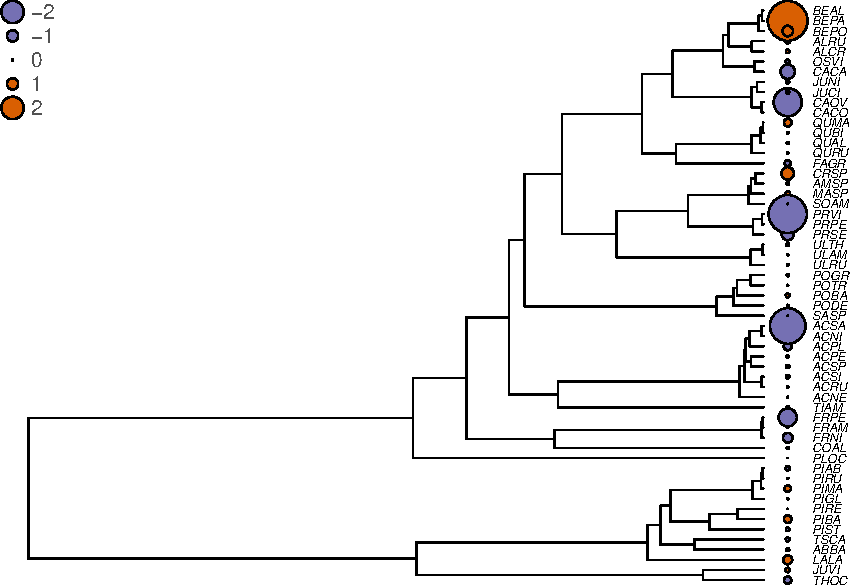
\includegraphics{pcm-workshop_files/figure-latex/Challenge 3 - solution-1.pdf}

\begin{Shaded}
\begin{Highlighting}[]
\FunctionTok{par}\NormalTok{(op)}
\end{Highlighting}
\end{Shaded}

\section{Challenge 4}\label{challenge-4-1}

Try to fit a PGLS with a Pagel correlation structure when regressing Shade tolerance on seed mass. Are the residuals as phylogenetically correlated than in the previous regression with wood density?

\begin{Shaded}
\begin{Highlighting}[]
\CommentTok{\# Fit a PGLS with the gls function}
\NormalTok{Sm.pgls2 }\OtherTok{\textless{}{-}} \FunctionTok{gls}\NormalTok{(Shade }\SpecialCharTok{\textasciitilde{}}\NormalTok{ Sm, }\AttributeTok{data =}\NormalTok{ seedplantsdata, }\AttributeTok{correlation=}\NormalTok{pagel.corr)}
\CommentTok{\# Get the results}
\FunctionTok{summary}\NormalTok{(Sm.pgls2)}
\end{Highlighting}
\end{Shaded}

\begin{verbatim}
## Generalized least squares fit by REML
##   Model: Shade ~ Sm 
##   Data: seedplantsdata 
##        AIC      BIC    logLik
##   187.6889 195.7183 -89.84447
## 
## Correlation Structure: corPagel
##  Formula: ~Code 
##  Parameter estimate(s):
##   lambda 
## 0.951553 
## 
## Coefficients:
##                  Value Std.Error   t-value p-value
## (Intercept)  2.8204268  1.497276  1.883705  0.0649
## Sm          -0.0000716  0.000060 -1.193604  0.2378
## 
##  Correlation: 
##    (Intr)
## Sm -0.009
## 
## Standardized residuals:
##        Min         Q1        Med         Q3        Max 
## -0.6946682 -0.3115198  0.1068607  0.2604470  0.8319385 
## 
## Residual standard error: 2.620527 
## Degrees of freedom: 57 total; 55 residual
\end{verbatim}

  \bibliography{book.bib}

\end{document}
